\documentclass[paper=a4,11pt,titlepage,twoside=true,headings=normal,numbers=noenddot,captions=tableabove,listof=totoc,index=totoc,bibliography=totoc]{scrreprt}
%\usepackage{amsmath} % abgesetzte Formeln zentriert in der Zeile
%\usepackage[fleqn,intlimits]{amsmath} % [fleqn] abgesetzte Formeln mit festem Abstand zum linken Rand
\usepackage[reqno,intlimits]{amsmath} % [reqno] um die gleichungsnummerierung rechts zu haben
% intlimits: Grenzen für Integrale unterhalb und oberhalb des Zeichens
\usepackage{amssymb}
\usepackage{array}
%\usepackage[ngerman]{babel}
%\usepackage[ngerman]{varioref}
\usepackage[english]{babel}
\usepackage[english]{varioref}
\usepackage[T1]{fontenc} 
\usepackage[utf8]{inputenc}
%---------------------------
\usepackage{booktabs}
\usepackage{calc}
\usepackage{cancel}
\usepackage[labelfont={footnotesize,sf,bf},textfont={footnotesize,sf}]{caption} %Format (Textgröße, Textform) für Bildtext 
%normalsize
%scriptsize
% sc --> smallcaps
% bf --> bold face
% sf --> sans serif
%\usepackage{cite} %inkompatibel mit biblatex
\usepackage[table]{xcolor}
%\usepackage{colortbl}
\usepackage[right]{eurosym}
%\usepackage{caption2} %nicht zusammen mit sidecap
%\usepackage{exscale}
\usepackage{ellipsis}
\usepackage{graphicx}
\usepackage{float}
%\usepackage{floatflt}
%----------------------------------------
\usepackage{gensymb} %-----------
%\usepackage{helvet}
\usepackage{csquotes}
\usepackage{listings}
\usepackage{longtable}
\usepackage{lastpage}  %----------
\usepackage{lscape}
\usepackage{lmodern}  %-- Silbentrennung
%\usepackage{mathpazo} % andere mathematische Symbol
\usepackage{makeidx}
%\usepackage{minitoc}
\usepackage{multirow}
\usepackage{multicol}
%\usepackage[intoc]{nomencl}   % zwei Spalten beim Formelzeichenverzeichnis
%\usepackage[german,intoc]{nomentbl} %vier Spalten bei Formelzeichenverzeichnis
\usepackage[english,intoc]{nomentbl} %vier Spalten bei Formelzeichenverzeichnis
\usepackage{nicefrac} %----
%\usepackage{picins} %----------
\usepackage{paralist} %--------
\usepackage{parallel}  %----------
\usepackage{pdfpages} %-------
% Define user colors using the RGB model
%\usepackage{colortbl}
%\definecolor{dunkelgrau}{rgb}{0.8,0.8,0.8}
%\definecolor{hellgrau}{rgb}{0.95,0.95,0.95}
%\usepackage{pgfplots}
\usepackage[figuresright]{rotating} 
\usepackage{scrlayer-scrpage}
%\usepackage[innercaption]{sidecap} %Beschriftung neben Bild, Tabelle, Mittelbach S333 %----------
%\usepackage{sistyle}
%\usepackage[locale=DE]{siunitx} %nicht zusammen mit sistyle %---------
\usepackage[locale=DE,per-mode=symbol,parse-numbers=false]{siunitx} %nicht zusammen mit sistyle %---------
\usepackage[font={scriptsize,sl},captionskip=3pt]{subfig} % für die Unterbilder %---------
\usepackage{shortvrb}
\usepackage{tablefootnote}
\usepackage{tabularx}
\usepackage{tabulary}
\usepackage{textcomp}
\usepackage{tocbasic}
%\usepackage{tikz}
\usepackage{times} 
\usepackage{units} %----------
\usepackage{url}
\usepackage{wrapfig} %----------
\usepackage{xr-hyper}
\usepackage{arydshln} %für \hdashline[5pt/2pt] % muss am Ende stehen, sonst gibt es Probleme mit xcolor
\usepackage{hyperref} % muss am Schluss stehen
\hypersetup{linkcolor={0 1 1}, linkbordercolor={1 1 1}, citebordercolor={1 1 1}} % setzt Linkboxen auf Farbe "`weiß"'
%\usepackage{bm}
%\usepackage[toc,symbols]{glossaries} %---------- muss nach hyperref stehen
\usepackage[nonumberlist, acronym, toc, section]{glossaries} % muss nach hypersetup stehen
%----------------
%\usepackage{romannum} % Seitenzahlen in römischen Ziffern
%\usepackage{adjustbox}
\usepackage{scrhack}
\usepackage[style=phys, citestyle=numeric, backend=biber]{biblatex}
\usepackage[useregional]{datetime2}
\usepackage{cleveref} % löscht labels!!!!!!!!!! <--- warum? habs trotzdem eingefügt weil es die referencen nice macht ohne newcommands dafür zu brauchen. außerdem steht intellisense drauf ;)
\usepackage{isotope} % um chemische gleichungen hübscher darstellen zu können
%-------------------------
 %\renewcommand{\captionlabelfont}{\sffamily} %für "Abbildung" und "Tabelle"
 %\renewcommand{\captionfont}{\sffamily\small} %für den Text der Bildunterschriften
%  \renewcommand{\captionlabelfont}{\sffamily} 
%  \renewcommand{\captionfont}{\sffamily} %\renewcommand{\normalfont}{\sffamily} %für die Überschriften
% Fettdruck der Bezeichnung Abbildung, Tabelle
%\renewcommand{\captionlabelfont}{\bfseries}
%---------------------------------------------
%------------------ Schrifttyp in der Kopf- und Fusszeilen
\setkomafont{pageheadfoot}{\footnotesize\sffamily}
%---------------------------------------------------
%Ändern der Abbildung- und Tabellenbezeichnung (Niedermair S.157)
%_____________________________________________
\addto\captionsngerman{\renewcommand\figurename{Abb.}}
\addto\captionsngerman{\renewcommand\tablename{Tab.}}
\renewcommand\listfigurename{Abbildungen}
%_______________________________
%Betrag eines Wertes
% \newcommand{\abs}[1]{\lvert #1 \rvert}
%---------------------------------------------
% \newcommand{\absatz}[1]{\textbf{\textsc{#1}}} %siehe Mittelbach S. 876ff
%----------------------------
%\newcommand{\absatz}{\par \medskip}
%______________________________
%\newcommand{\anhang}[1]{Anhang \ref{#1}, Seite \pageref{#1}}
% \newcommand{\anhang}[1]{Anhang \vref{#1}}
% %________________________________
% \newcommand{\aufgabe}{\stepcounter{plus} Aufgabe \arabic{plus}}
%______________________________________
%compactitem
% \newcommand{\bci}{\begin{compactitem}}
% \newcommand{\eci}{\end{compactitem}}
% %______________________________________
% %
% \newcommand{\bi}{\begin{itemize}}
% \newcommand{\ei}{\end{itemize}}
% %______________________________________
% %compactenumerate
% \newcommand{\bce}{\begin{compactenum}}
% \newcommand{\ece}{\end{compactenum}}
% %_____________________________________
% %begin equation
% \newcommand{\be}{\begin{equation}}
% \newcommand{\ee}{\end{equation}}
% %_____________________________________
% %begin equation ohne Formelnummer
% \newcommand{\ben}{\begin{equation*}}
% \newcommand{\een}{\end{equation*}}
% %_____________________________________
% %begin align ohne Formelnummer
% \newcommand{\ban}{\begin{align*}}
% \newcommand{\ean}{\end{align*}}
%_____________________________________
%begin align
% \newcommand{\ba}{\begin{align}}
% \newcommand{\ea}{\end{align}}
%_____________________________________
%minpage
% \newcommand{\bmp}{\begin{minipage}[t]{.47\linewidth}}
% \newcommand{\emp}{\end{minipage}}
%_____________________________
%  dB
% \newcommand{\db}{dB}
% %  dB(A)
% \newcommand{\dba}{ dB(A) }
% %  dB(A) für Satzende
% \newcommand{\dbap}{ dB(A)}
% %_________________________________
% \newcommand{\bzw}{bzw.\,}
% %_______________________________
% \newcommand{\dif}{\mathrm{d}}
%________________________________
% neuer Zähler
\newcounter{plus}
\setcounter{plus}{0}
%______________________________
%Für das Formelverzeichnis _____________________ Formelverzeichis ____
% Befehl umbenennen in fz
% \let\fz\nomenclature
% Deutsche Überschrift
\renewcommand{\nomname}{Formelzeichen}
% Punkte zw. Abkürzung und Erklärung
\setlength{\nomlabelwidth}{.20\hsize}
\renewcommand{\nomlabel}[1]{#1 \dotfill}
% Zeilenabstände verkleinern
\setlength{\nomitemsep}{-\parsep}
%_____________________________
% \newcommand{\bild}[1]{Abb. \vref{#1}}
% \newcommand{\sbild}[1]{siehe Abb. \vref{#1}}
% \newcommand{\bilder}[2]{Abb. \vrefrange{#1}{#2}}
% \newcommand{\bildseite}[1]{Abb. \vref{#1}} % erzeugt "`Abb. nn auf Seite nn
% \newcommand{\tabelle}[1]{Tab. \vref{#1}}
% \newcommand{\tabellenseite}[1]{Tab. \vref{#1}} % erzeugt "`Tab. nn auf Seite nn
% für \vref ist usepackage[german]{varioref} einzufügen
%_-------------------------------- Freiraum
% \newcommand{\freiraum}[1]{\begin{figure}[H]\vspace{#1\textheight}\end{figure}}
%_____________________________
% Gleichung
% \newcommand{\gl}[1]{Gl.\,(\ref{#1})}
% \newcommand{\sgl}[1]{siehe Gl.\,(\ref{#1})}
% \newcommand{\glbereich}[2]{Gl. \vrefrange[]{#1}{#2}}
%_____________________________
% Grad Celsius
% \newcommand{\grad}{\,\degC}
% \newcommand{\gradC}{\,\degree}
%______________________________________
% Großbuchstaben als Indizes kleiner schreiben; spezielle im Mathemodus
% \newcommand{\klein}[1]{\scriptscriptstyle{#1}}% Fettdruck der Bezeichnung 
%______________________________
%% Kasten
% \newcommand{\kasten}{\fbox{\rule{0.0pt}{10pt}{{ } } }}
%______________________________
%\newcommand{\kapitel}[1]{Kapitel \ref{#1}, Seite \pageref{#1}}
% \newcommand{\kapitel}[1]{Kapitel \vref{#1}}
%_____________________________
%  LAeq für den äquivalenten Dauerschallpegel
% \newcommand{\laeq}{ $L_{Aeq}$ }
%  LAeq für den äquivalenten Dauerschallpegel am Satzende
% \newcommand{\laeqp}{ $L_{Aeq}$}
%_________________________________
%   Linie zeichnen
\newcommand{\linie}{\rule{0.5\textwidth}{0.1pt}}
%---------------------- LaTeX
% \newcommand{\lt}{\LaTeX\,\,}
%----------------------------
% \newcommand{\nl}{\newline}
%__________________________________
%  multicolumn für Tabellen
% \newcommand{\mc}{\multicolumn}
%% \mc{1}{c}{Text}
%_________________________________
%    Parallel
% \newcommand{\pl}[1]{\ParallelLText{#1}}
% \newcommand{\pr}[1]{\ParallelRText{#1}}
% \newcommand{\pp}{\ParallelPar}
%------------ rot unterstrichen
% \newcommand{\rotunterstrichen}[1]{\textcolor{red}{\underline{\textcolor{black}{#1}}}}
%________________ Realteil
% \newcommand{\real}[1]{\text{Re}\left\{#1\right\}}
%________________________________--
% \newcommand{\seite}[1]{Seite \pageref{#1}}
% \newcommand{\seiten}[2]{\vpagerefrange{#1}{#2}}
%----------------------------
%        TEXT Rot
\newcommand{\textrot}[1]{\textcolor{red}{#1}}
%______________________________
%Abkürzung für \multicolumn
% \newcommand{\tab}[2]{\multicolumn{1}{#1}{#2}}
%_____________________________________
% doppelt unterstreichen
% \newcommand{\unterstreichen}[1]{\underline{\underline{#1}}}
% einfach unterstreichen
% \newcommand{\ul}[1]{\underline{#1}}
%______________________________
%kurze Verbatimausgabe
%\MakeShortVerb{\|} %mittelbach S.160 mit \usepackage{shortvrb}
%_______________________________________
% vspace
% \newcommand{\vsf}{\vspace{5pt}}
%_________________________________
% \newcommand{\zb}{z.B.\,}
% \newcommand{\idr}{i.d.R.\,}
%_______________________________
% Zähler-einfach
\newcounter{req}
% \newcommand{\zaehler}[1]{\refstepcounter{req}{#1} \thereq}
%% Beispielaufzählung \zaehler{Beispiel}\\
%_____________________________________
 \setlength{\voffset}{-2.532 cm}
 \setlength{\hoffset}{-1.57 cm}
% \setlength{\topmargin}{2.0 cm} \setlength{\topskip}{0.1 cm}
 \setlength{\topmargin}{1.5 cm}
 \setlength{\topskip}{0.1 cm}
 \setlength{\evensidemargin}{1.5 cm}
 \setlength{\oddsidemargin}{1.5 cm}
 \setlength{\textwidth}{16.5 cm}
 \setlength{\footskip}{40pt}
 \setlength{\textheight}{24.5cm}
% \setlength{\textheight}{23.5 cm}
 \setcounter{page}{1}
 \setlength{\parindent}{0cm}
 \setlength{\headsep}{20pt}
%----------------------------------------------------------------------
% Linien in der Kopf- und Fußzeile
%\renewcommand{\headrulewidth}{0.0pt}   %Linie in der Kopfzeile mit 0.0pt keine Linie
%%\renewcommand{\footrulewidth}{0.0pt}   %Linie in der Fußzeile mit 0.0 pt keine Linie
%\renewcommand{\headrulewidth}{0.2pt}   %Linie in der Kopfzeile mit 0.0pt keine Linie
%\renewcommand{\footrulewidth}{0.2pt}   %Linie in der Fußzeile mit 0.0 pt keine Linie
%------------------------------------------------------------------------
%\renewcommand{\normalfont}{\sffamily} %für die Überschriften
%\renewcommand{\chaptermark}[1]{\markboth{\chaptername\ \thechapter #1}{}}
%\renewcommand{\sectionmark}[1]{\markright{\thesection\ #1}}
% \rfoot{\leftmark\\\rightmark}

%Definitionen für Kopfzeile
% bei documentclass {report} hat der Eintrag für die [gerade Seite] keine Wirkung
%-------------------------------------------------------------
%%
%Einstellungen für Kopf- und Fusszeilen mit dem KOMA-Skript und \usepackage{scrpage2}
\pagestyle{scrheadings}
%\pagestyle{scrplain}
% le --> links, gerade Seite
% ce --> mittig, gerade Seite
% re --> rechts, gerade Seite
% lo --> links, ungerade Seite
% co --> mittig, ungerade Seite
% ro --> rechts, ungerade Seite
%---------------------------------------------
% Löschen aller Einträge
%\clearscrheadings
% \automark[section]{subsection}
% \pagemark --> Seitenzahl
% \automark --> Kapitelüberschriften
% \leftmark --> ??
% \rightmark --> ??
%::::::::::::::::::::::::::::::::::: Kopfzeile
% Kopfzeile gerade Seite
\automark[chapter]{chapter}
\lehead[]{\titelkopfzeilelinkseven}
\cehead[]{\titelkopfzeilemitteeven}
\rehead[]{\titelkopfzeilerechtseven}
% Kopfzeile ungerade Seite
\lohead[]{\titelkopfzeilelinksodd}
\cohead[]{\titelkopfzeilemitteodd}
\rohead[]{\titelkopfzeilerechtsodd}
% Linie in der Kopfzeile
%\setheadtopline{0.2pt} % obere Linie in der Kopfzeile; nur bei scrartcl
%\setheadsepline{0.4pt} % untere Linie in der Kopfzeile; nur bei scrartcl
\KOMAoptions{headsepline=0.4pt}
% Linie in der Fusszeile
%::::::::::::::::::::::::::::::::::: Fußzeile
% Fusszeile gerade Seite[plain-style]{scrheadings-style}
\lefoot[]{\titelfusszeilelinkseven} 
\cefoot[]{\titelfusszeilemitteeven}
\refoot[]{\titelfusszeilerechtseven}
% Fusszeile ungerade Seite
\lofoot[]{\titelfusszeilelinksodd}
\cofoot[]{\titelfusszeilemitteodd}
\rofoot[]{\titelfusszeilerechtsodd}
%\rofoot[\thepage ]{\thepage}
%\setfoottopline{0.2pt} % obere Linie in der Kopfzeile; nur bei scrartcl
%\setfootsepline{0.4pt} % untere Linie in der Kopfzeile; nur bei scrartcl
\KOMAoptions{footsepline=0.4pt}

% le --> links, gerade Seite
% ce --> mittig, gerade Seite
% re --> rechts, gerade Seite
% lo --> links, ungerade Seite
% co --> mittig, ungerade Seite
% ro --> rechts, ungerade Seite
% even --> gerade Seite
% odd --> ungerade Seite
%----------------------------------------- Kopfzeilentext
 \newcommand{\titelkopfzeilemitteeven}{}
 \newcommand{\titelkopfzeilemitteodd}{}
 \newcommand{\titelkopfzeilelinkseven}{Hochschule RheinMain}
 \newcommand{\titelkopfzeilelinksodd}{}
 \newcommand{\titelkopfzeilerechtseven}{}
 \newcommand{\titelkopfzeilerechtsodd}{Hochschule RheinMain}
 %----------------------------------------- Fußzeilentext
 \newcommand{\titelfusszeilemitteeven}{}
 \newcommand{\titelfusszeilemitteodd}{}
 \newcommand{\titelfusszeilerechtseven}{Studienbereich Angewandte Physik \& Medizintechnik}
 \newcommand{\titelfusszeilerechtsodd}{\thepage \hspace{0.5mm} von \pageref{LastPage}}
 \newcommand{\titelfusszeilelinkseven}{\thepage \hspace{0.5mm} von \pageref{LastPage}}
 \newcommand{\titelfusszeilelinksodd}{Studienbereich Angewandte Physik \& Medizintechnik}
\newcommand{\titelLV}{Physics Lab 3}
%---------------------------- VARIABLEN festlegen ------------------
%----------- Pro Versuch zu ändernde Angaben -----------------------
\newcommand{\versuch}{2} % Versuchsnummer einfügen
\newcommand{\untertitelb}{Signal Propagation in Coaxial Cables} % Titel des Versuchs einfügen
\newcommand{\datumLV}{17.11.2020} % Datum einfügen
\newcommand{\deadline}{1.12.2020} % Abgabedatum ist der 1.12.2020
\newcommand{\dateLVa}{Dezember 1st, 2020}
\newcommand{\dateLVb}{Dezember 8th, 2020}
%----------- TITEL
\newcommand{\untertitela}{Experiment P3-2}
% -------- Student 1
\newcommand{\nameA}{Cihan Ünlü}
% --------- Student 2
\newcommand{\nameB}{Dennis Hunter}
% --------- Student 3, falls vorhanden
\newcommand{\nameC}{Sebastian Kreß}
%::::::::::::::::::::::::::::::::::
%\input{chapters/glossar}
%\renewcommand\USenglishtoday
\DeclareNameAlias{author}{last-first}
\DeclareNameAlias{editor}{last-first}
\DeclareNameAlias{translator}{last-first}
\addbibresource{quellen.bib}
\begin{document}%\selectlanguage{USenglish}
%-----------------------------------------------------------------
\begin{titlepage} 
	\newcommand{\HRule}{\rule{\linewidth}{0.5mm}} 	
	\centering
	\textsc{\Large Hochschule RheinMain} \par
	\begin{center}
		
\includegraphics[width=0.15\textwidth]{logo-hsrm.jpg}
	\end{center}%\vspace{.5cm}
%	\textsc{\Large Hochschule RheinMain}\vspace{1cm]
	\textsc{\LARGE \titelLV}\vspace{0.5cm}
		\HRule\vspace{0.4cm}
	{\huge\bfseries \untertitela}\par\vspace{0.4cm} % Titel des Dokuments
	{\huge\bfseries \untertitelb}\par\vspace{0.4cm} % Titel des Dokuments
		\HRule\vspace{1.5cm}
%-------------------
%\begin{flushleft}
	\begin{minipage}{0.4\textwidth}
%	\begin{flushleft}
%\centering
		\large
		\textit{\underline{Authors}}\par\vspace{0.5cm}
		\textsc{\nameA}\par\vspace{0.5cm}
		\textsc{\nameB}\par\vspace{0.5cm}
		\textsc{\nameC}\par\vspace{0.5cm}
		%\textsc{\nameC}\vspace{0.5cm] 
%	\end{flushleft}
\end{minipage}
%------------------------------------
\vfill\vfill\vfill 
%\textsc{\Large Fachbereich Ingenieurwissenschaften}\vspace{0.5cm]
\textsc{\Large Department of Engineering}\par\vspace{0.5cm}
%\textsc{\large Studienbereich Angewandte Physik \& Medizintechnik}\vspace{0.5cm]
\textsc{\large Applied Physics \& Medical Technology}\par\vspace{0.5cm}
\vfill
\begin{tabular}{ll}
	Date of experiment:\hspace{0.4cm} &{\large\dateLVa}\\
	Date of submission:\hspace{0.4cm} &{\large\today} 
\end{tabular}
\end{titlepage}

%-----------------------------------------------------
\tableofcontents
\newpage
%--------------------
\chapter{Introduction}
%
\section{Terms and Definitions}
    \subsection*{Transmission Line}\label{sec:transmissionLine}
    %
    In there simplest form cables are made out of a conducting material to transport electrical energy or signals from point
    A to point B. The higher the frequency of the signal to transmit, the less the wave nature of can be neglected.
    %
    \subsection*{Characteristic Impedance, Velocity Factor and Propagation Speed}
    %
    Characteristic impedance: The impedance, when connected to a transmission line, suppresses any reflections and standing
    waves \cite{ATIS.AmericanTelecomStandards2001}.
    Velocity factor: Relative signal propagation speed inside a transmission line expressed as percent of speed of light.
    Propagation speed: The absolute speed at which a signal propagates through a medium.
    %
    \subsection*{Time Domain Reflectometry}
    %
    A method to inspect properties of a transmission line i.e. length, characteristic impedance and velocity factor as
    well as the presence, nature and location of defects.
    %
    \subsection*{Avalanche Pulse Generator}
    %
    A circuit to generate ultra short pulses on a scale of picoseconds. Its main working principle abuses the avalanche
    breakdown of a transistor across the collector-emitter line. The breakdown voltage is usually much higher than the
    voltages during normal operation.
    %
    \subsection*{Boost Converter}
    %
    A circuit capable of \textit{boosting} a constant current input voltage to a much higher output voltage by repeatedly
    switching an inductor on and off. The fly back voltage induced by the break down of the magnetic field gets stored in
    a capacitance and forms the voltage at the output terminals.
    %
    \subsection*{Pulse Width Modulation}
    %
    A constant current switched on and off at a fixed frequency. The time the signal is considered high relatively to the
    period time is called the duty cycle.
    %
    \subsection*{Amplitude, Rise Time, Fall Time, Pulse Width}
    %
    Amplitude: In a wider sense a term used to characterize repeating phenomena. It is defined as a signals maximum deviation
    from its arithmetic mean value.\par
    Rise time: a technical term defined as the time it takes for a system to transition its output from \( 10\% \) to \( 90\% \)
    of an infinitesimal steep input signal.\par
    % Fall time:
    Pulse width: 
    %
    \subsection*{Bandwidth and Rise Time of an Oscilloscope}
    %
    Text
    %
\section{Preparation}
%
    \subsection*{Reflection on a Transmission Line}
    %
    \begin{figure}[h]
        \centering
        \begin{framed}
            \textbf{!!! Insert Diagram Here !!!}
        \end{framed}
    \end{figure}
    %
    \subsection*{SPICE-Simulation of a Boost Converter}
    %
    \begin{figure}[h]
        \centering
        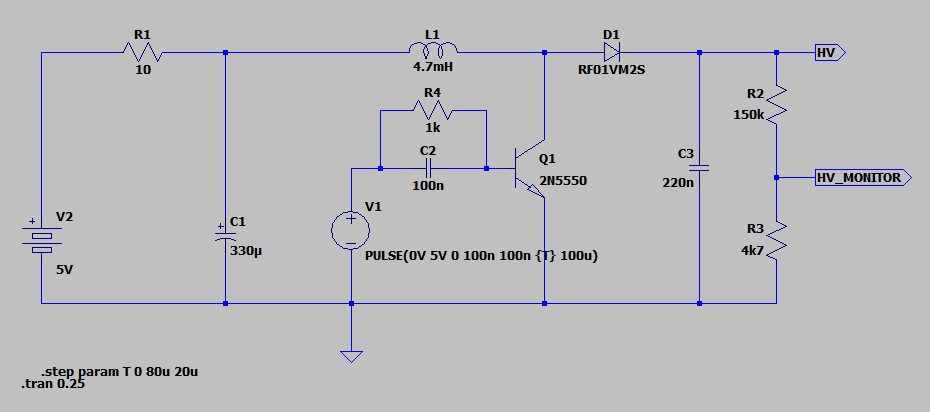
\includegraphics[width=\textwidth]{Spice/circuit.jpg}
        \caption[Simulated circuit of a boost converter.]{Simulated circuit of a boost converter using \textsc{LTspice}.}
        \label{fig:simCircuit}
    \end{figure}
    %
    \begin{figure}[h]
        \centering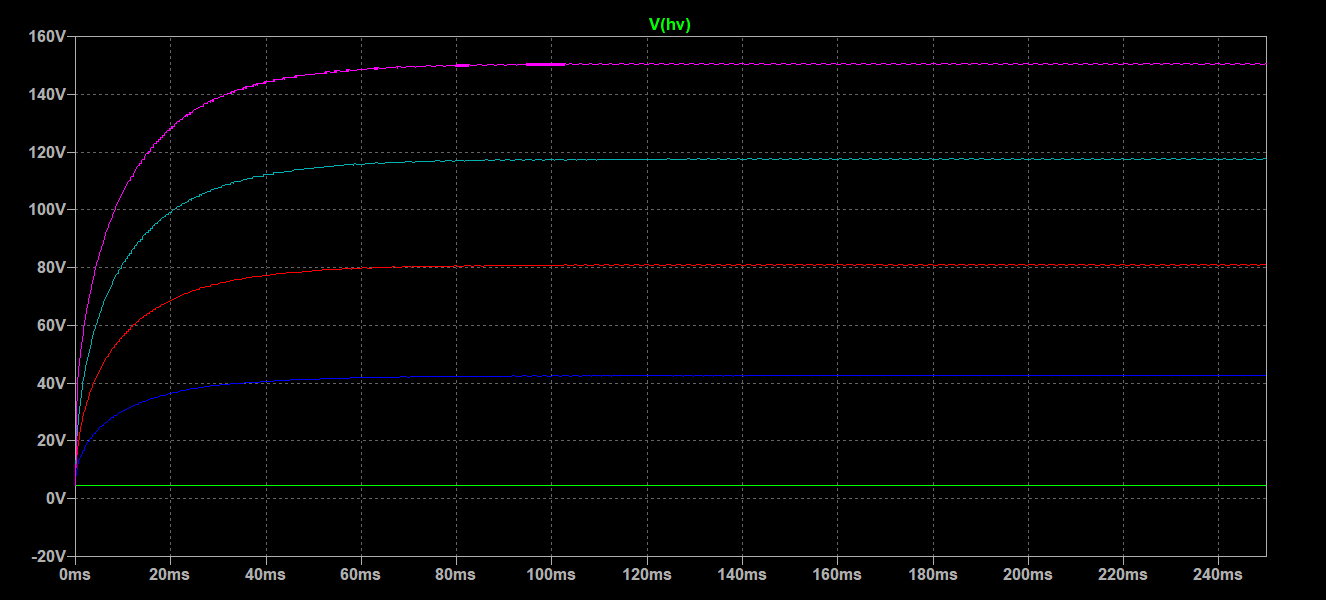
\includegraphics[width=\textwidth]{Spice/plot.jpg}
        \caption{Plot of the output voltage at \textit{HV}. The voltage is subsequently progressing towards a peak voltage of \( \hat{U}_{HV} \approx \SI[]{150}[]{V} \) with rising PWM duty cycle.}
        \label{fig:plotSimCircuit}
    \end{figure}
    %
    \subsection*{Charge/Discharge Time of a Capacitor}
    %
    Charging:
    \begin{gather}
        U_{Br} = U_+ \left( 1 - e^{-\frac{t_{charge}}{R_6C_5}}\right) \nonumber \\
        \Leftrightarrow \nonumber \\
        t_{charge} = - \ln\left(1 - \frac{U_{Br}}{U_+}\right) \cdot R_6 C_5
        \label{eq:avalanche_charging_equation}
    \end{gather}
    Discharging:
    \begin{gather}
        U_{C_5} = U_{Br} \left(e^{-\frac{t_{discharge}}{R_7C_5}}\right) \nonumber \\
        \Leftrightarrow \nonumber \\
        t_{discharge} = -\ln\left( \frac{U_{C_5}}{U_{Br}} \right) \cdot R_7 C_5
        \label{eq:avalanche_discharging_equation}
    \end{gather}
    plugging in the values for \(U_{Br} = \SI{65}{V}, U_+ = \SI{75}{V}, U_{C_5} = \SI{5}{V}, C_5 = \SI{2.2}{pF}, R_6 = \SI{1}{M\ohm} \text{ and } R_7 = \SI{51}{\ohm}\)
    equates to the following charging/discharging times \(t_{charge}\) and \(t_{discharge}\):
    \begin{align}
        t_{charge} &= - \ln\left(1 - \frac{\SI{65}{V}}{\SI{75}{V}}\right) \cdot \SI{10^6}{\ohm} \cdot \SI{2.2 \cdot 10^{-12}}{F} \nonumber \\
        &\approx \SI{4.43 \cdot 10^{-6}}{s} \label{eq:avalanche_charging_time}\\
        \nonumber \\
        t_{discharge} &= -\ln\left( \frac{\SI{5}{V}}{\SI{65}{V}} \right) \cdot \SI{51}{\ohm} \cdot \SI{2.2 \cdot 10^{-12}}{F} \nonumber \\
        &\approx \SI{2.88 \cdot 10^{-10}}{s} \label{eq:avalanche_discharging_time}
    \end{align}
    With these numbers, the minimum time per charge/discharge cycle would be the sum of both times. Thus, the maximum number
    of repetitions per second \(f_{Rep}\) is
    \begin{equation}
        f_{Rep} = \left(t_{charge} + t_{discharge}\right)^{-1} \approx \SI{225.7}{kHz}
    \end{equation}
    %
    \subsection*{Cable Characteristics of RG-58/U Coaxial Cable}% A4
    %
    Nominal characteristic impedance: \(\SI{53}{\ohm}\)\par
    Nominal velocity of propagation: \(69.5\%\)\par
    Nominal delay (translates to the inverse of the absolute speed of propagation): \(\SI{4.85588}{\nicefrac{ns}{m}}\)\par
    The values above are taken from the technical data sheet \cite{Belden.RG-58/U.CoaxCable.Datasheet}.
    %
    \subsection*{Determining the Suitability of the Oscilloscope}% A5
    %

    %
    \subsection*{Sampling Rate}% A6
    %
    %
\chapter{Set-Up of Experiment}
    To perform the experiment the elements shown in \cref{fig:setup} are needed. They are listed below.
    %
    \begin{figure}[h]
        \centering
        % \begin{framed}
            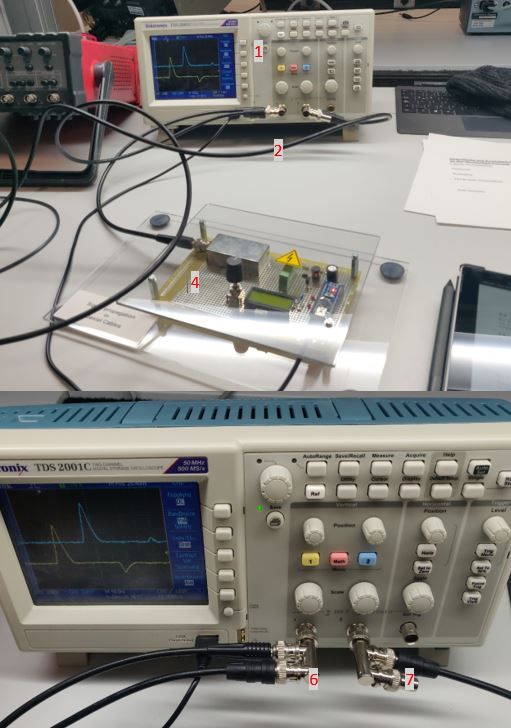
\includegraphics[width=.6\textwidth]{aufbau/setup_num.JPG}
        % \end{framed}
        %\includegraphics[width=12cm]{} % insert image (incl. numbering)
        \caption{Components needed for the experiment.}  
        \label{fig:setup}
    \end{figure}
    %
    \begin{enumerate}
        \item Oscilloscope
        \item Coaxial cables in three lengths
        % \item Coaxial cables with unknown length and internal fault
        \item Circuit board
        % \item Multimeter
        \item T-piece
        \item \SI{50}{\ohm} termination resistor
        % \item Termination box
        % \item Tape measure
    \end{enumerate}
    %
    A better overview of the circuit board will give the following \cref{fig:circuit_board}. Again, the components are listed
    below.
    %
    \begin{figure}[h]
        \centering
        % \begin{framed}
            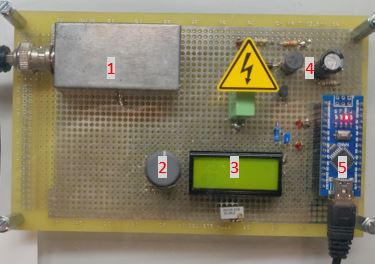
\includegraphics[width=.6\textwidth]{aufbau/circuit_board_num.JPG}
        % \end{framed}
        % \includegraphics[width=12cm]{} % insert image (incl. numbering)
        \caption{Detailed view on the circuit board.}  
        \label{fig:circuit_board}
    \end{figure}
    %
    \begin{enumerate}
        \item Pulse generator
        \item Potentiometer
        \item LCD
        \item Boost converter
        \item Arduino Nano Microcontroller board
    \end{enumerate}
    %
    The individual settings are explained in the execution chapter.
\input{chapters/4_durchführung}
\chapter{Evaluation}
\chapter{Conclusion}
%
%-------------------
\newpage
\listoffigures 
\listoftables
\addchap{List of Symbols}
\begin{table}[h]
    \begin{tabular}{@{}ll@{}}%
        \( A \) & Distinct event\\
    \end{tabular}
    \label{tab:glossar}
\end{table}
\appendix
\chapter{Appendix}
%
\begin{figure}[h]%
    \subfloat[Reference pulse at CH1. The delayed pulse is fed to CH2.\label{subfig:osci:ch1-ch2_delayed_pulse}]{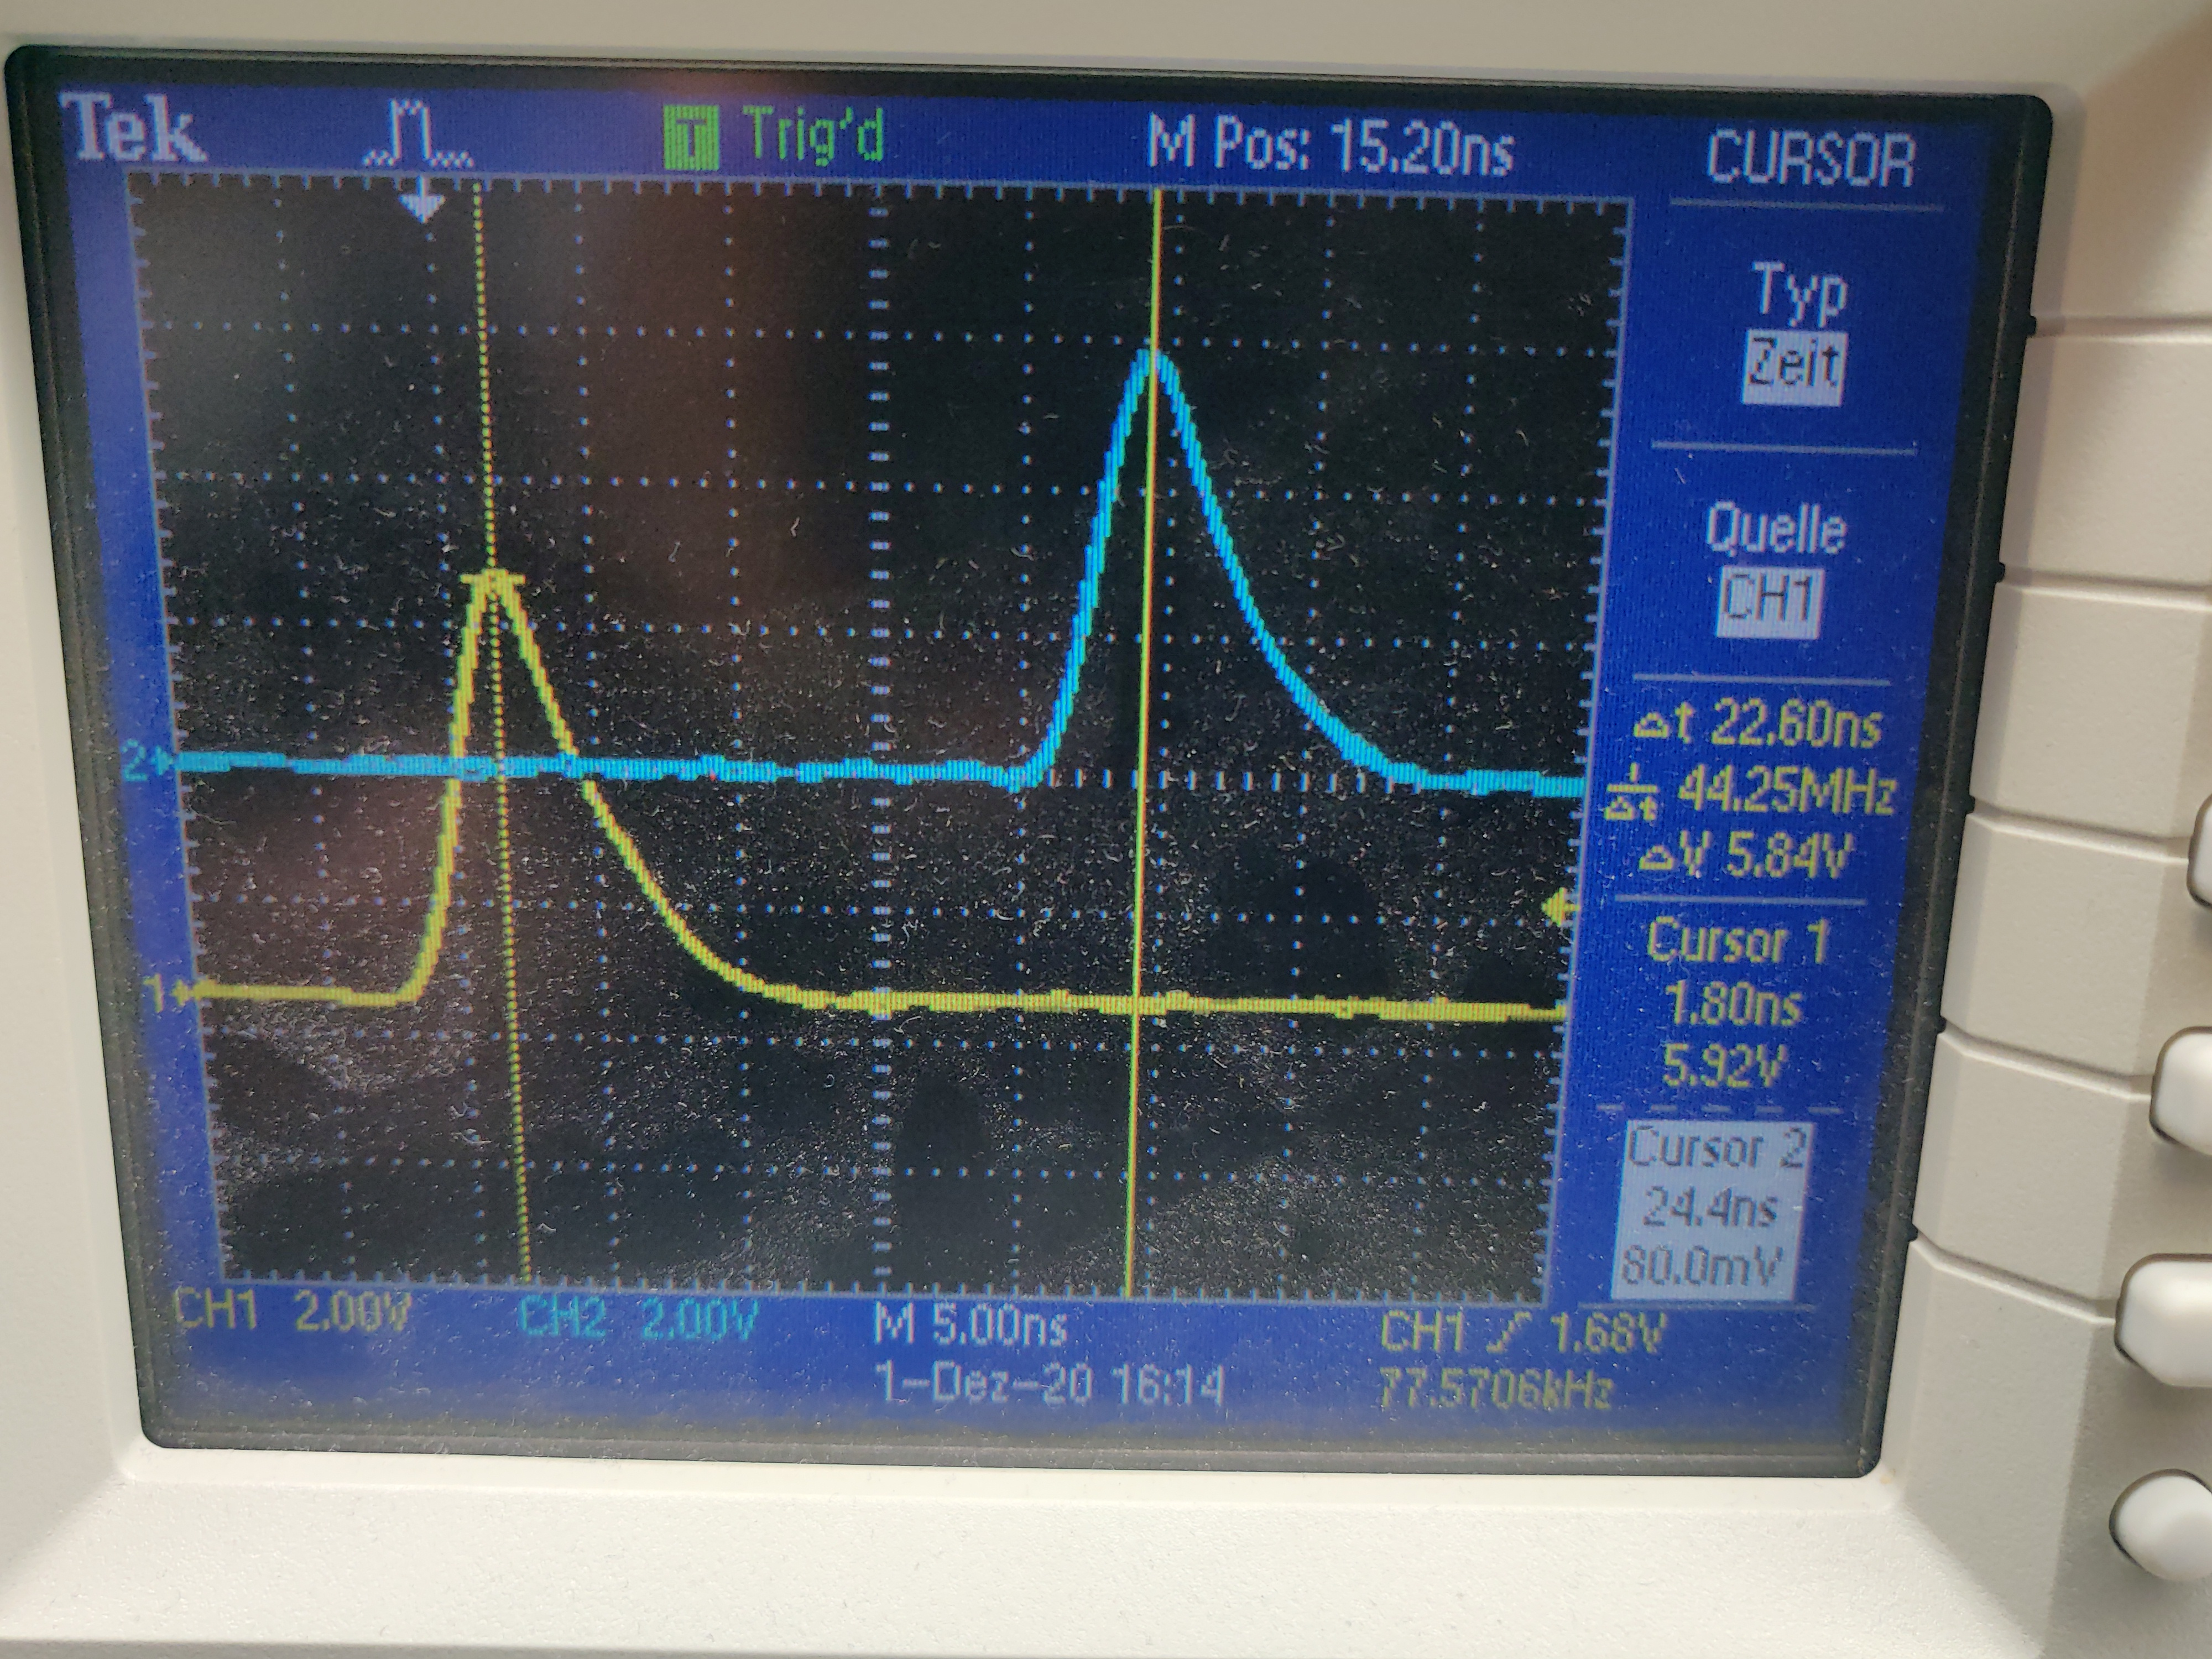
\includegraphics[width=0.45\linewidth]{messdaten/3-3-1_propagationDelay.jpg}}%
    \hspace{.05\linewidth}
    \subfloat[The reference pulse gets reflected at an open-ended cable connected to the same channel. A difference in time due to a finite propagation speed can be observed.\label{subfig:osci:3-3-2_open_reflectionTime}]{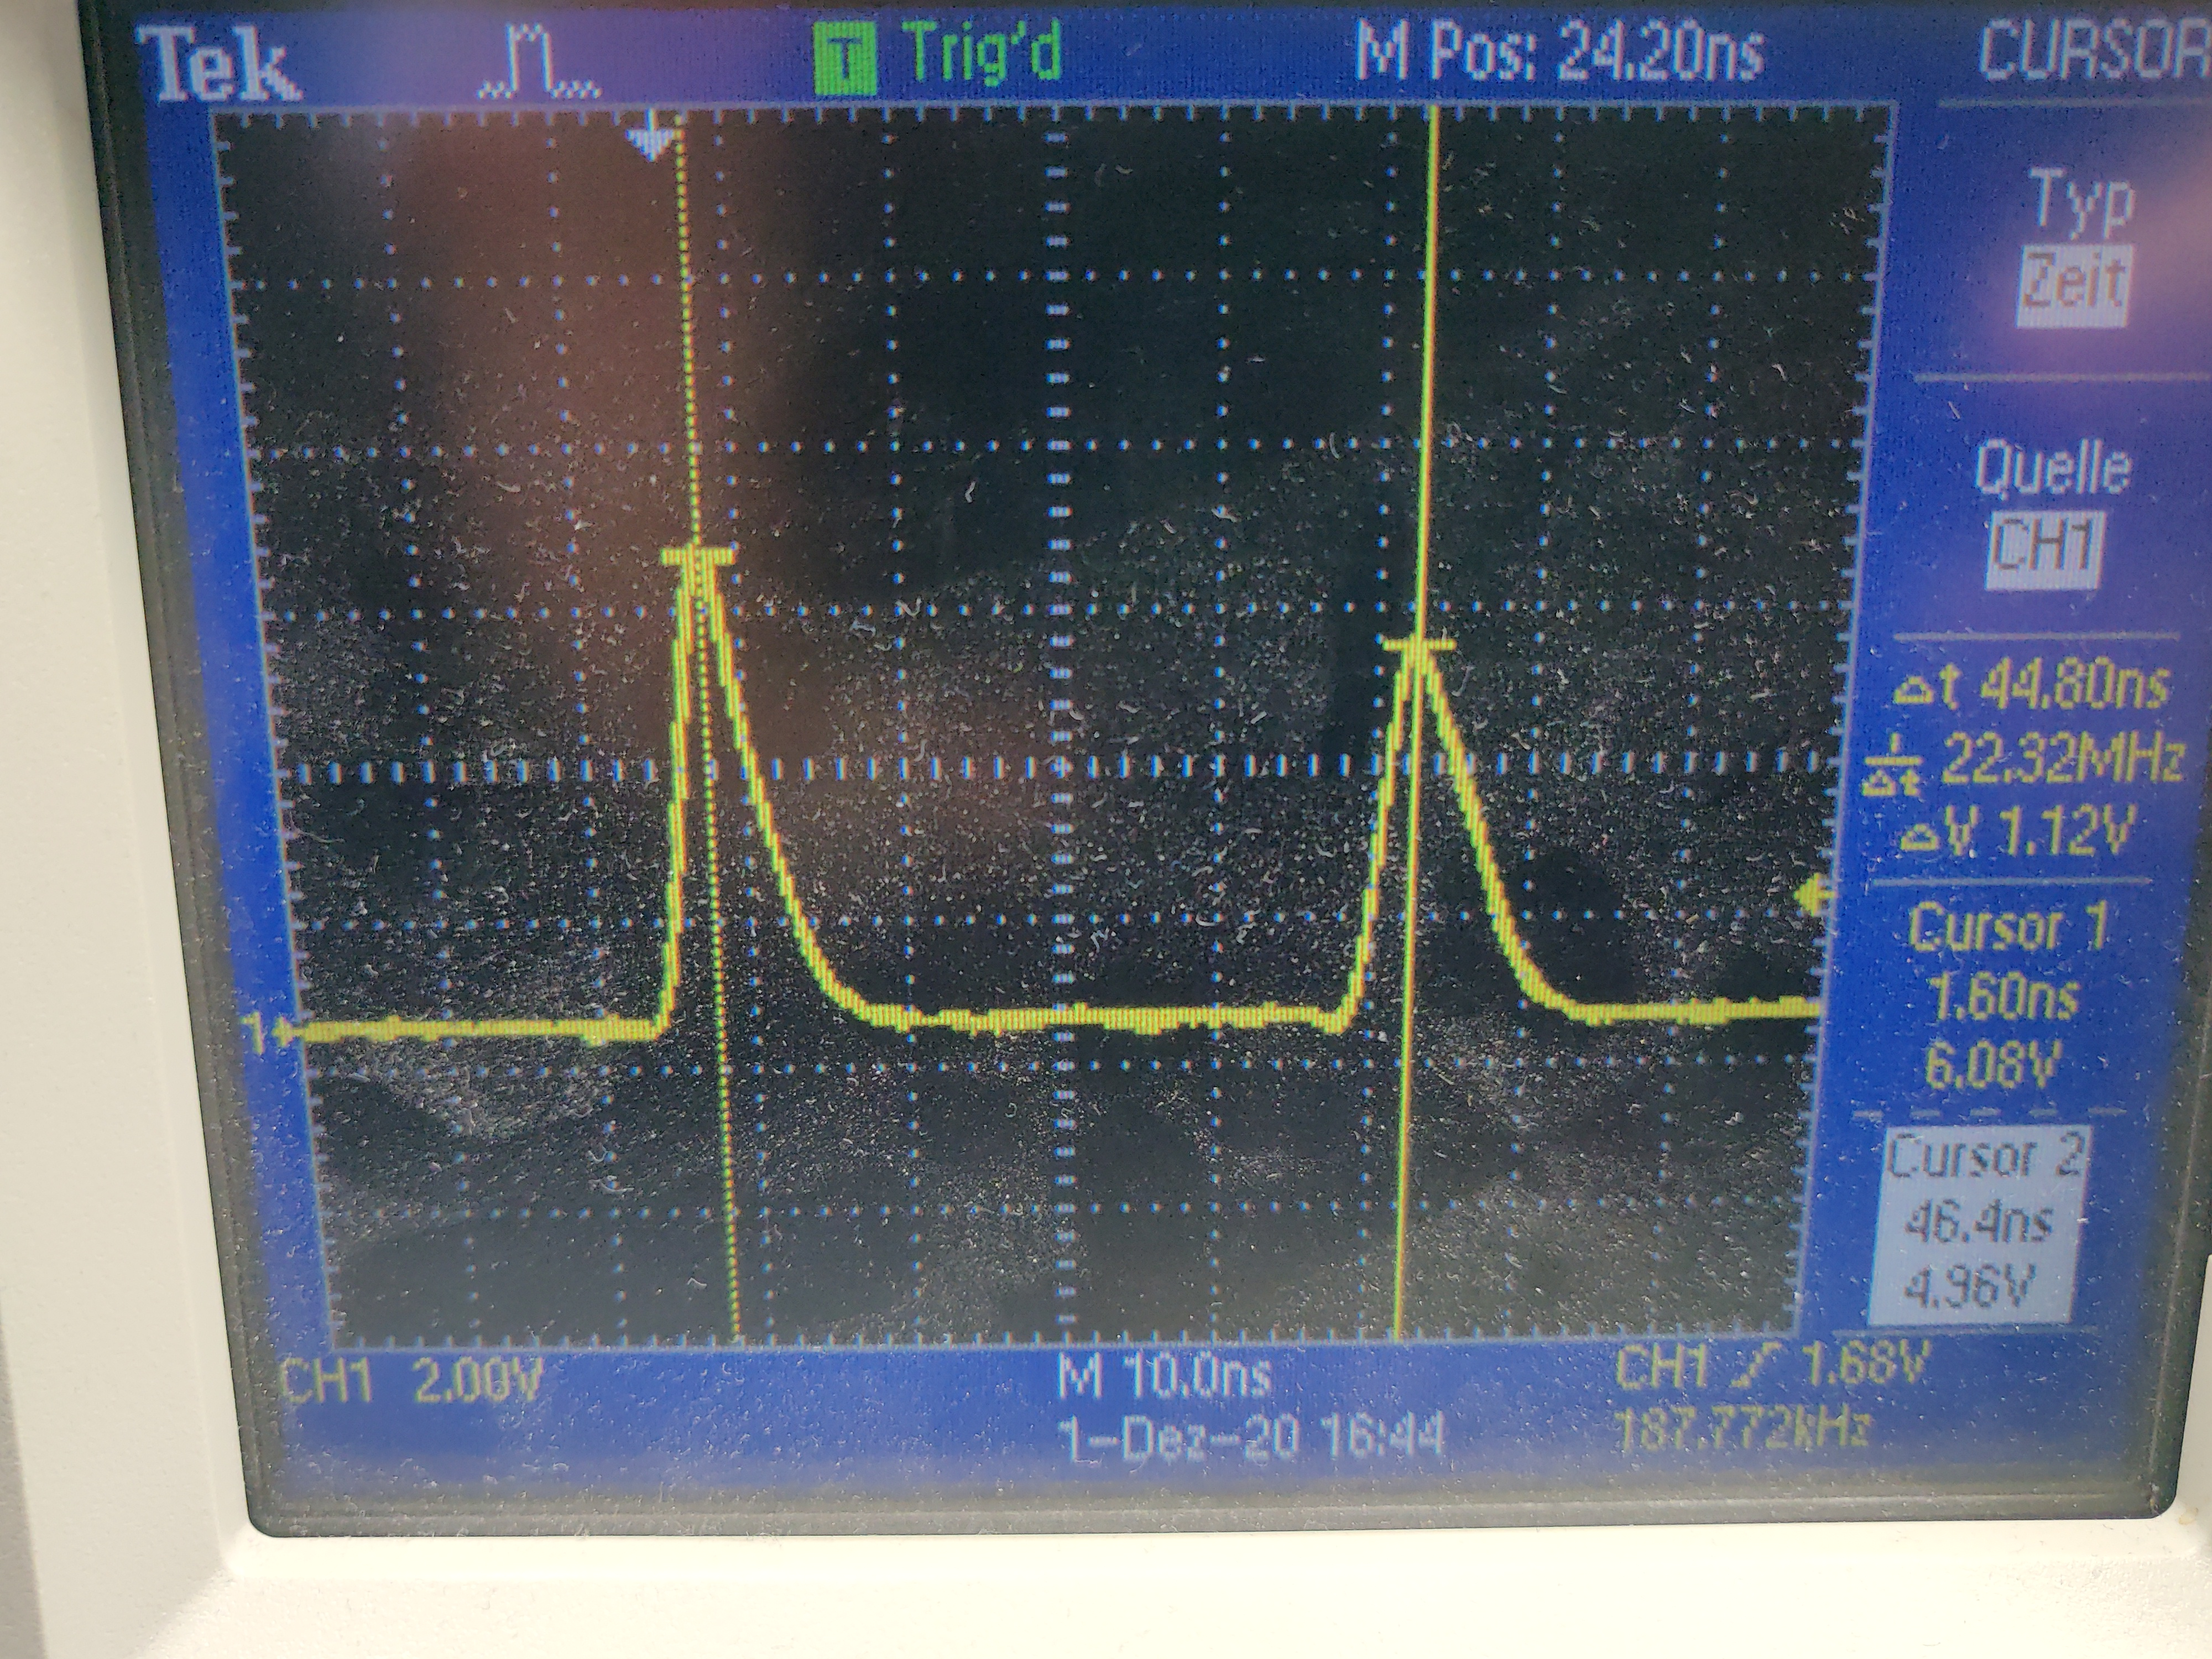
\includegraphics[width=0.45\linewidth]{messdaten/3-3-2_open_reflectionTime.jpg}}%
\end{figure}
\begin{figure}[h]\ContinuedFloat
    % \hspace{.05\linewidth}
    \subfloat[If the transmission line gets terminated with an impedance close to zero, the reflected pulse gets inverted.\label{subfig:osci:3-3-2_shorted}]{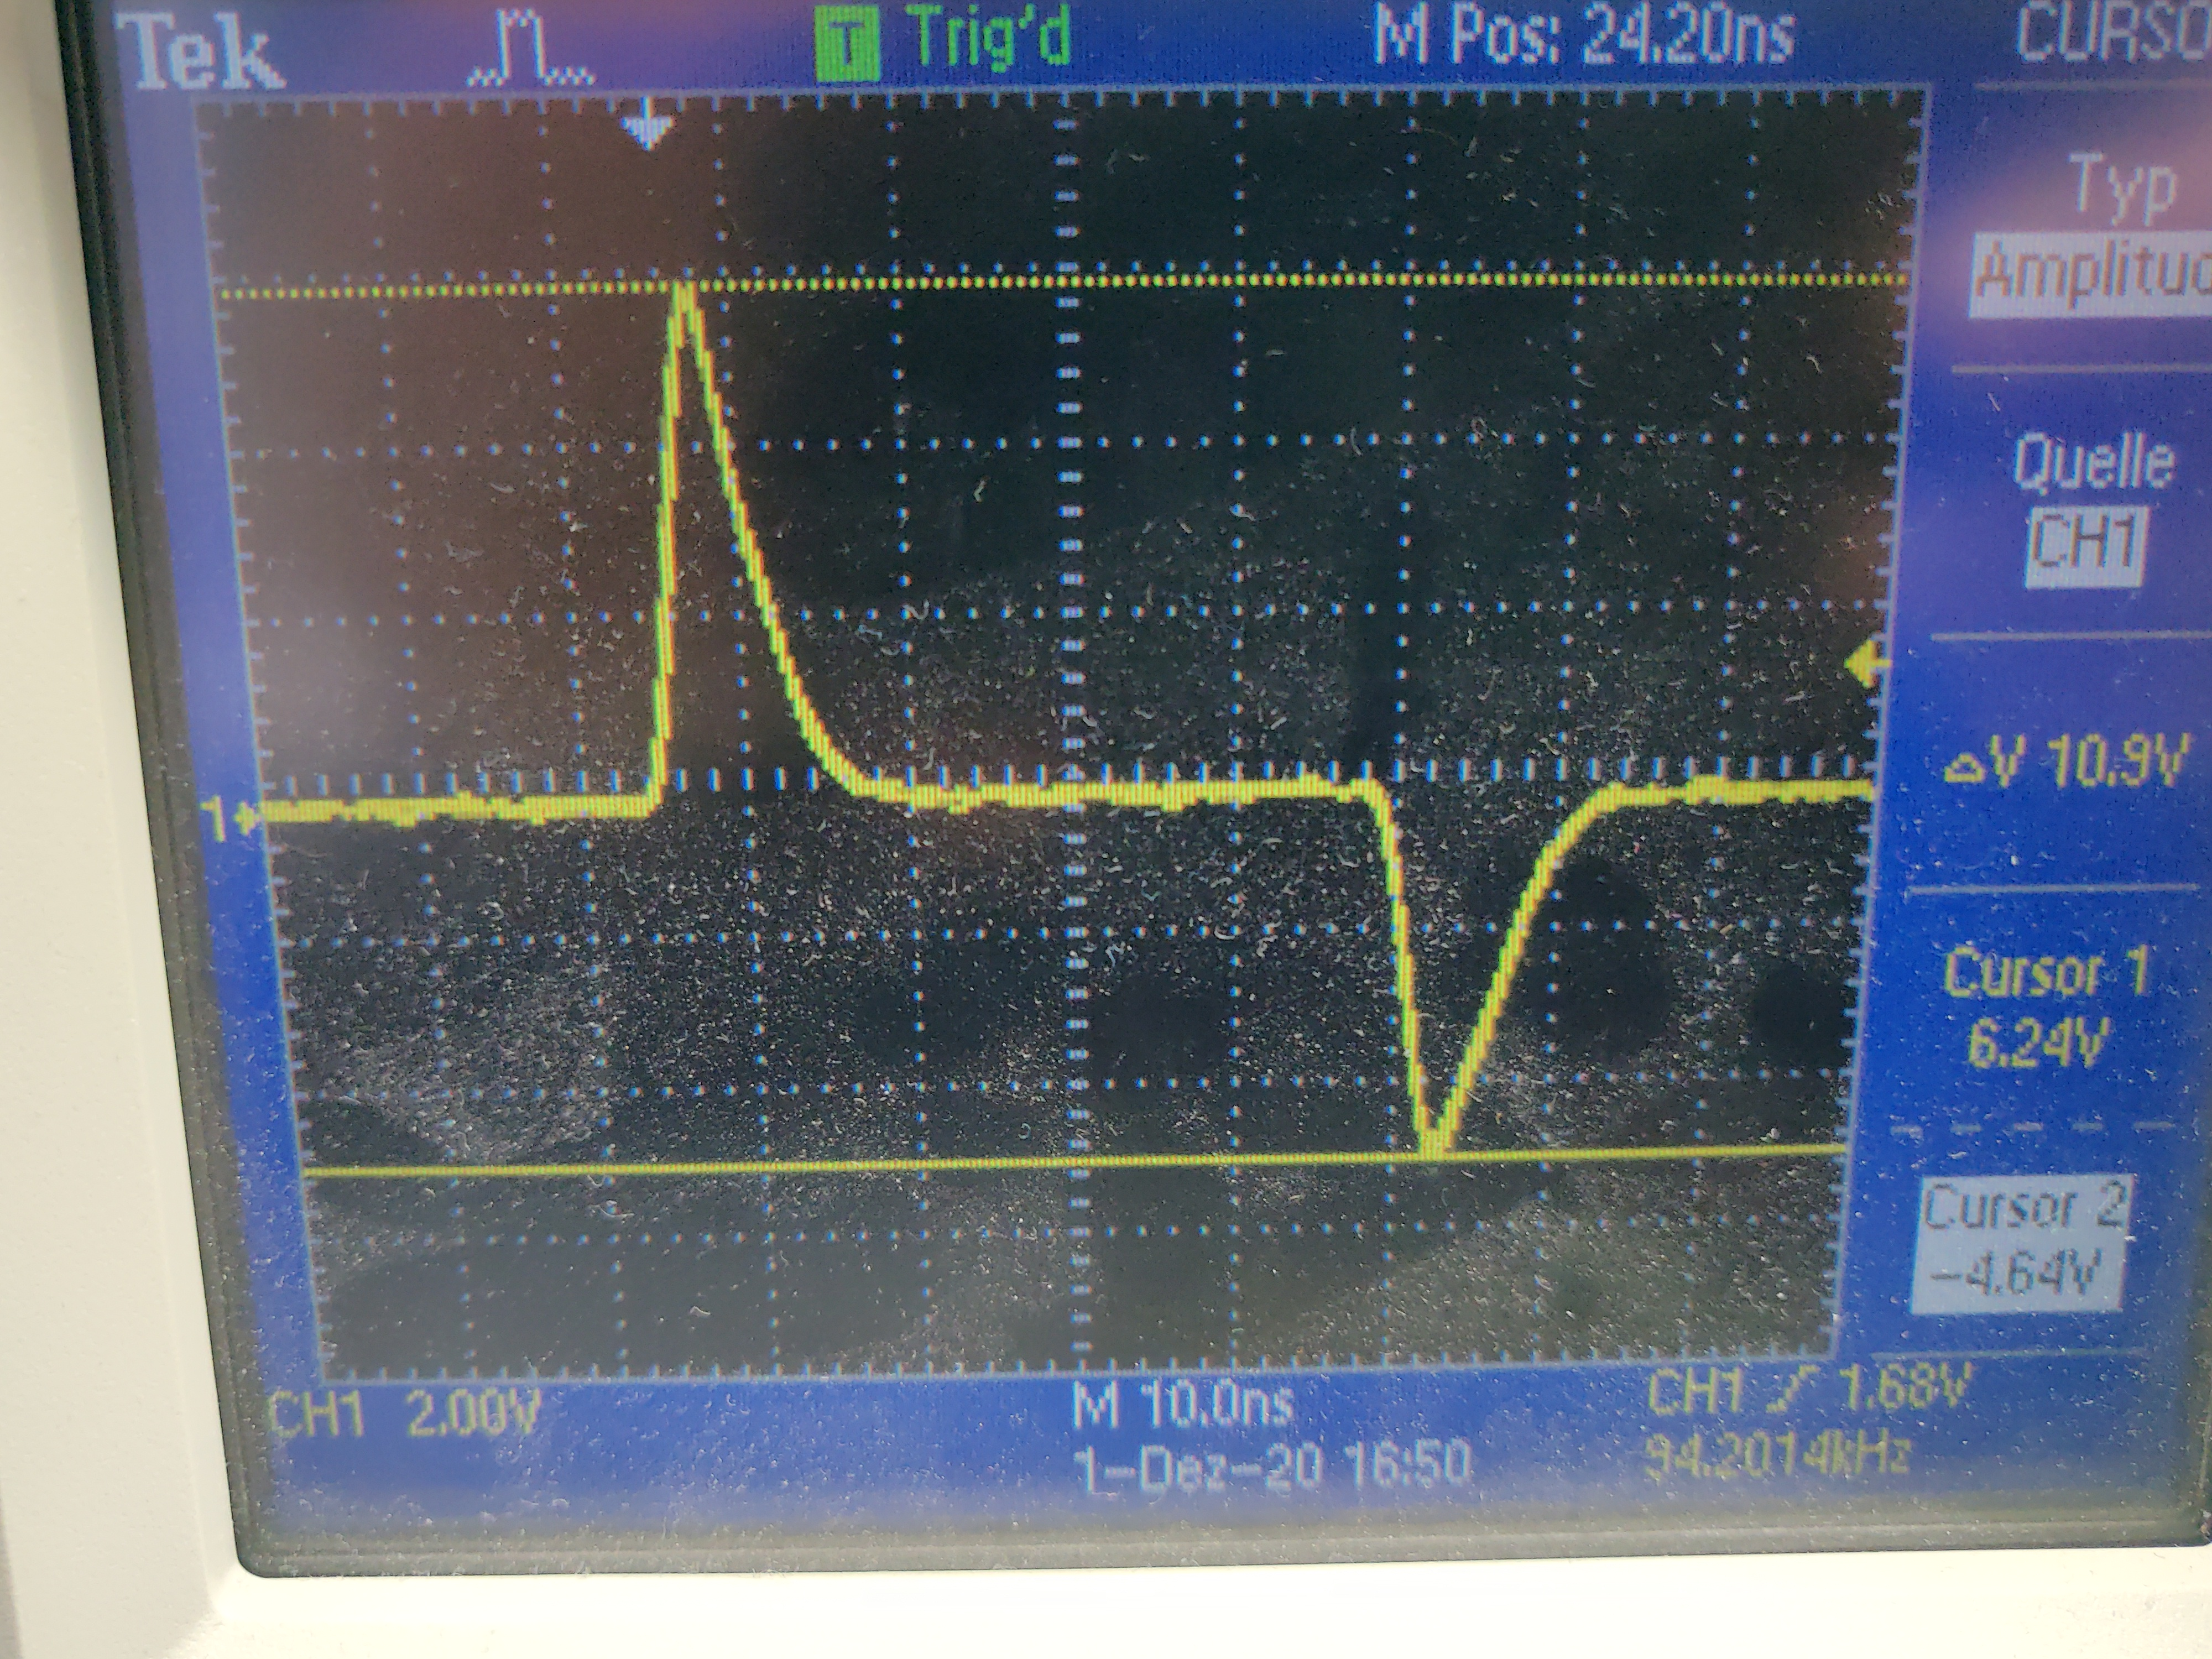
\includegraphics[width=0.45\linewidth]{messdaten/3-3-2_shorted.jpg}}%
    \hspace{.05\linewidth}
    \subfloat[The reflected signal can almost completely inhibited terminating the transmission line with an impedance close to its characteristic impedance.\label{subfig:osci:3-3-2_Z_0_equal_R_term}]{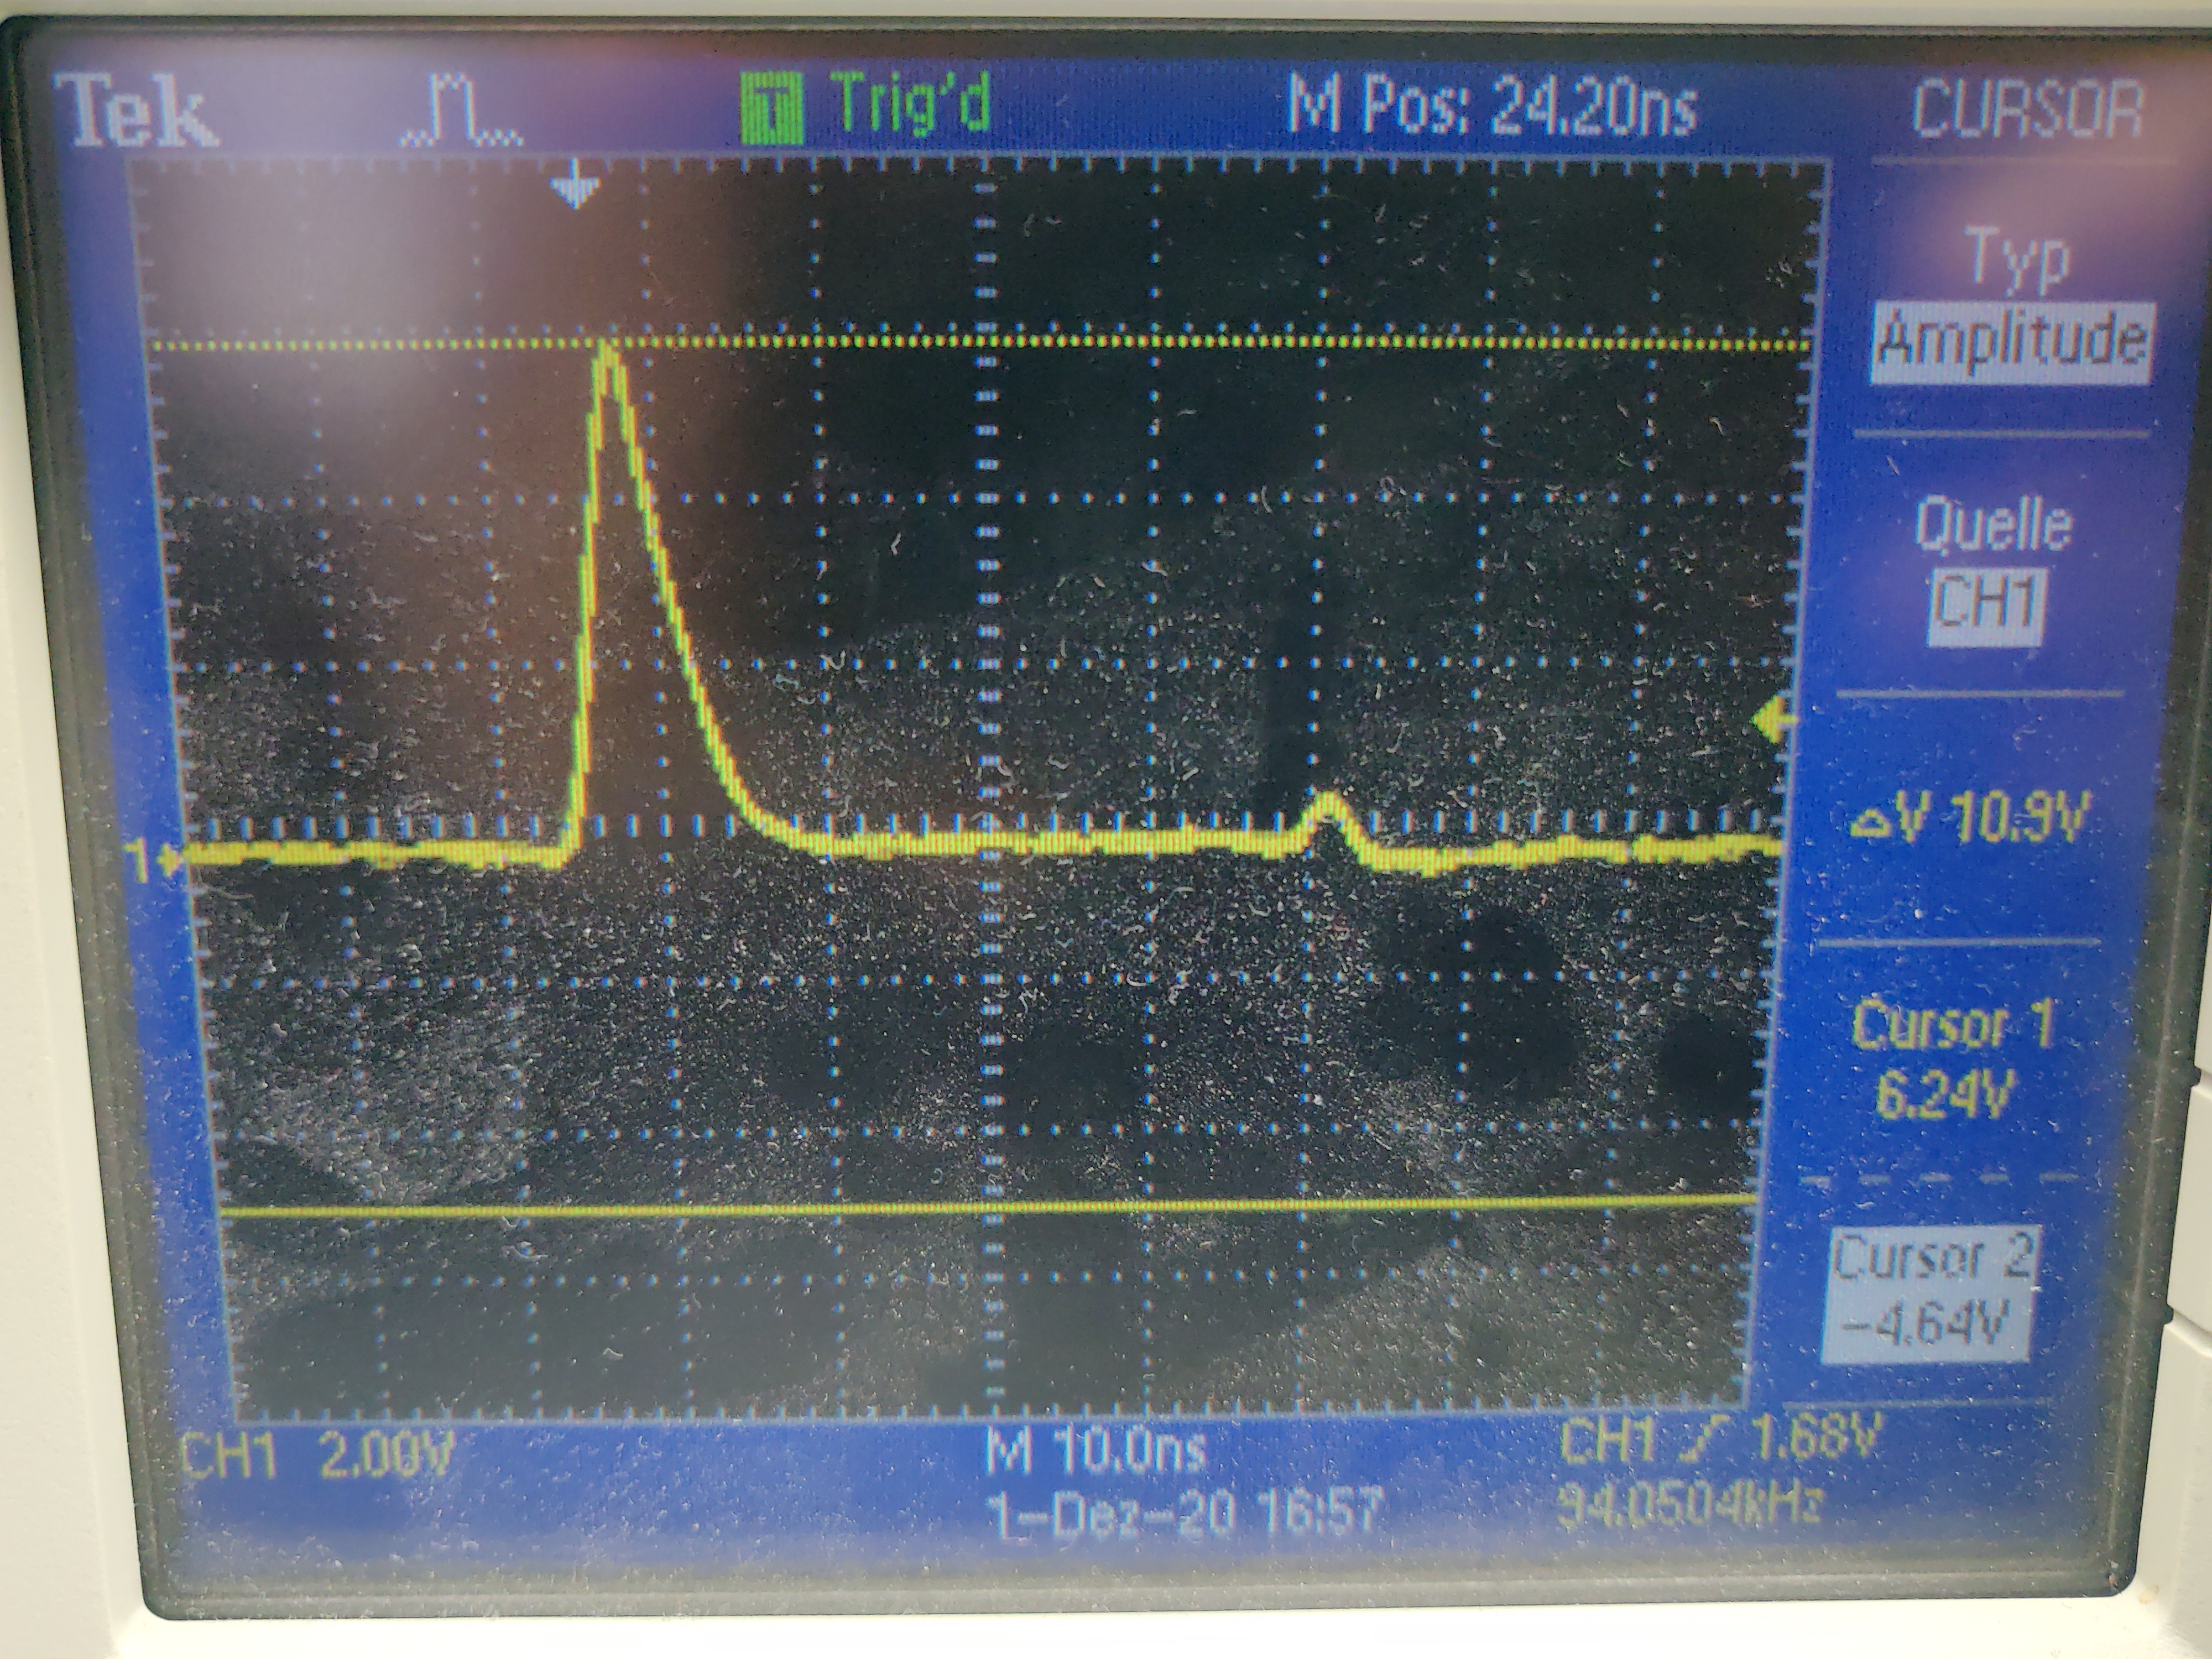
\includegraphics[width=0.45\linewidth]{messdaten/3-3-2_Z_0_equal_R_term.jpg}}%
\end{figure}
\begin{figure}[h]\ContinuedFloat
    \subfloat[Local changes to the cables characteristics reflect signals as well. This can be utilized to locate a defect along the cable's length.\label{subfig:osci:3-3-3_lengthToDefect}]{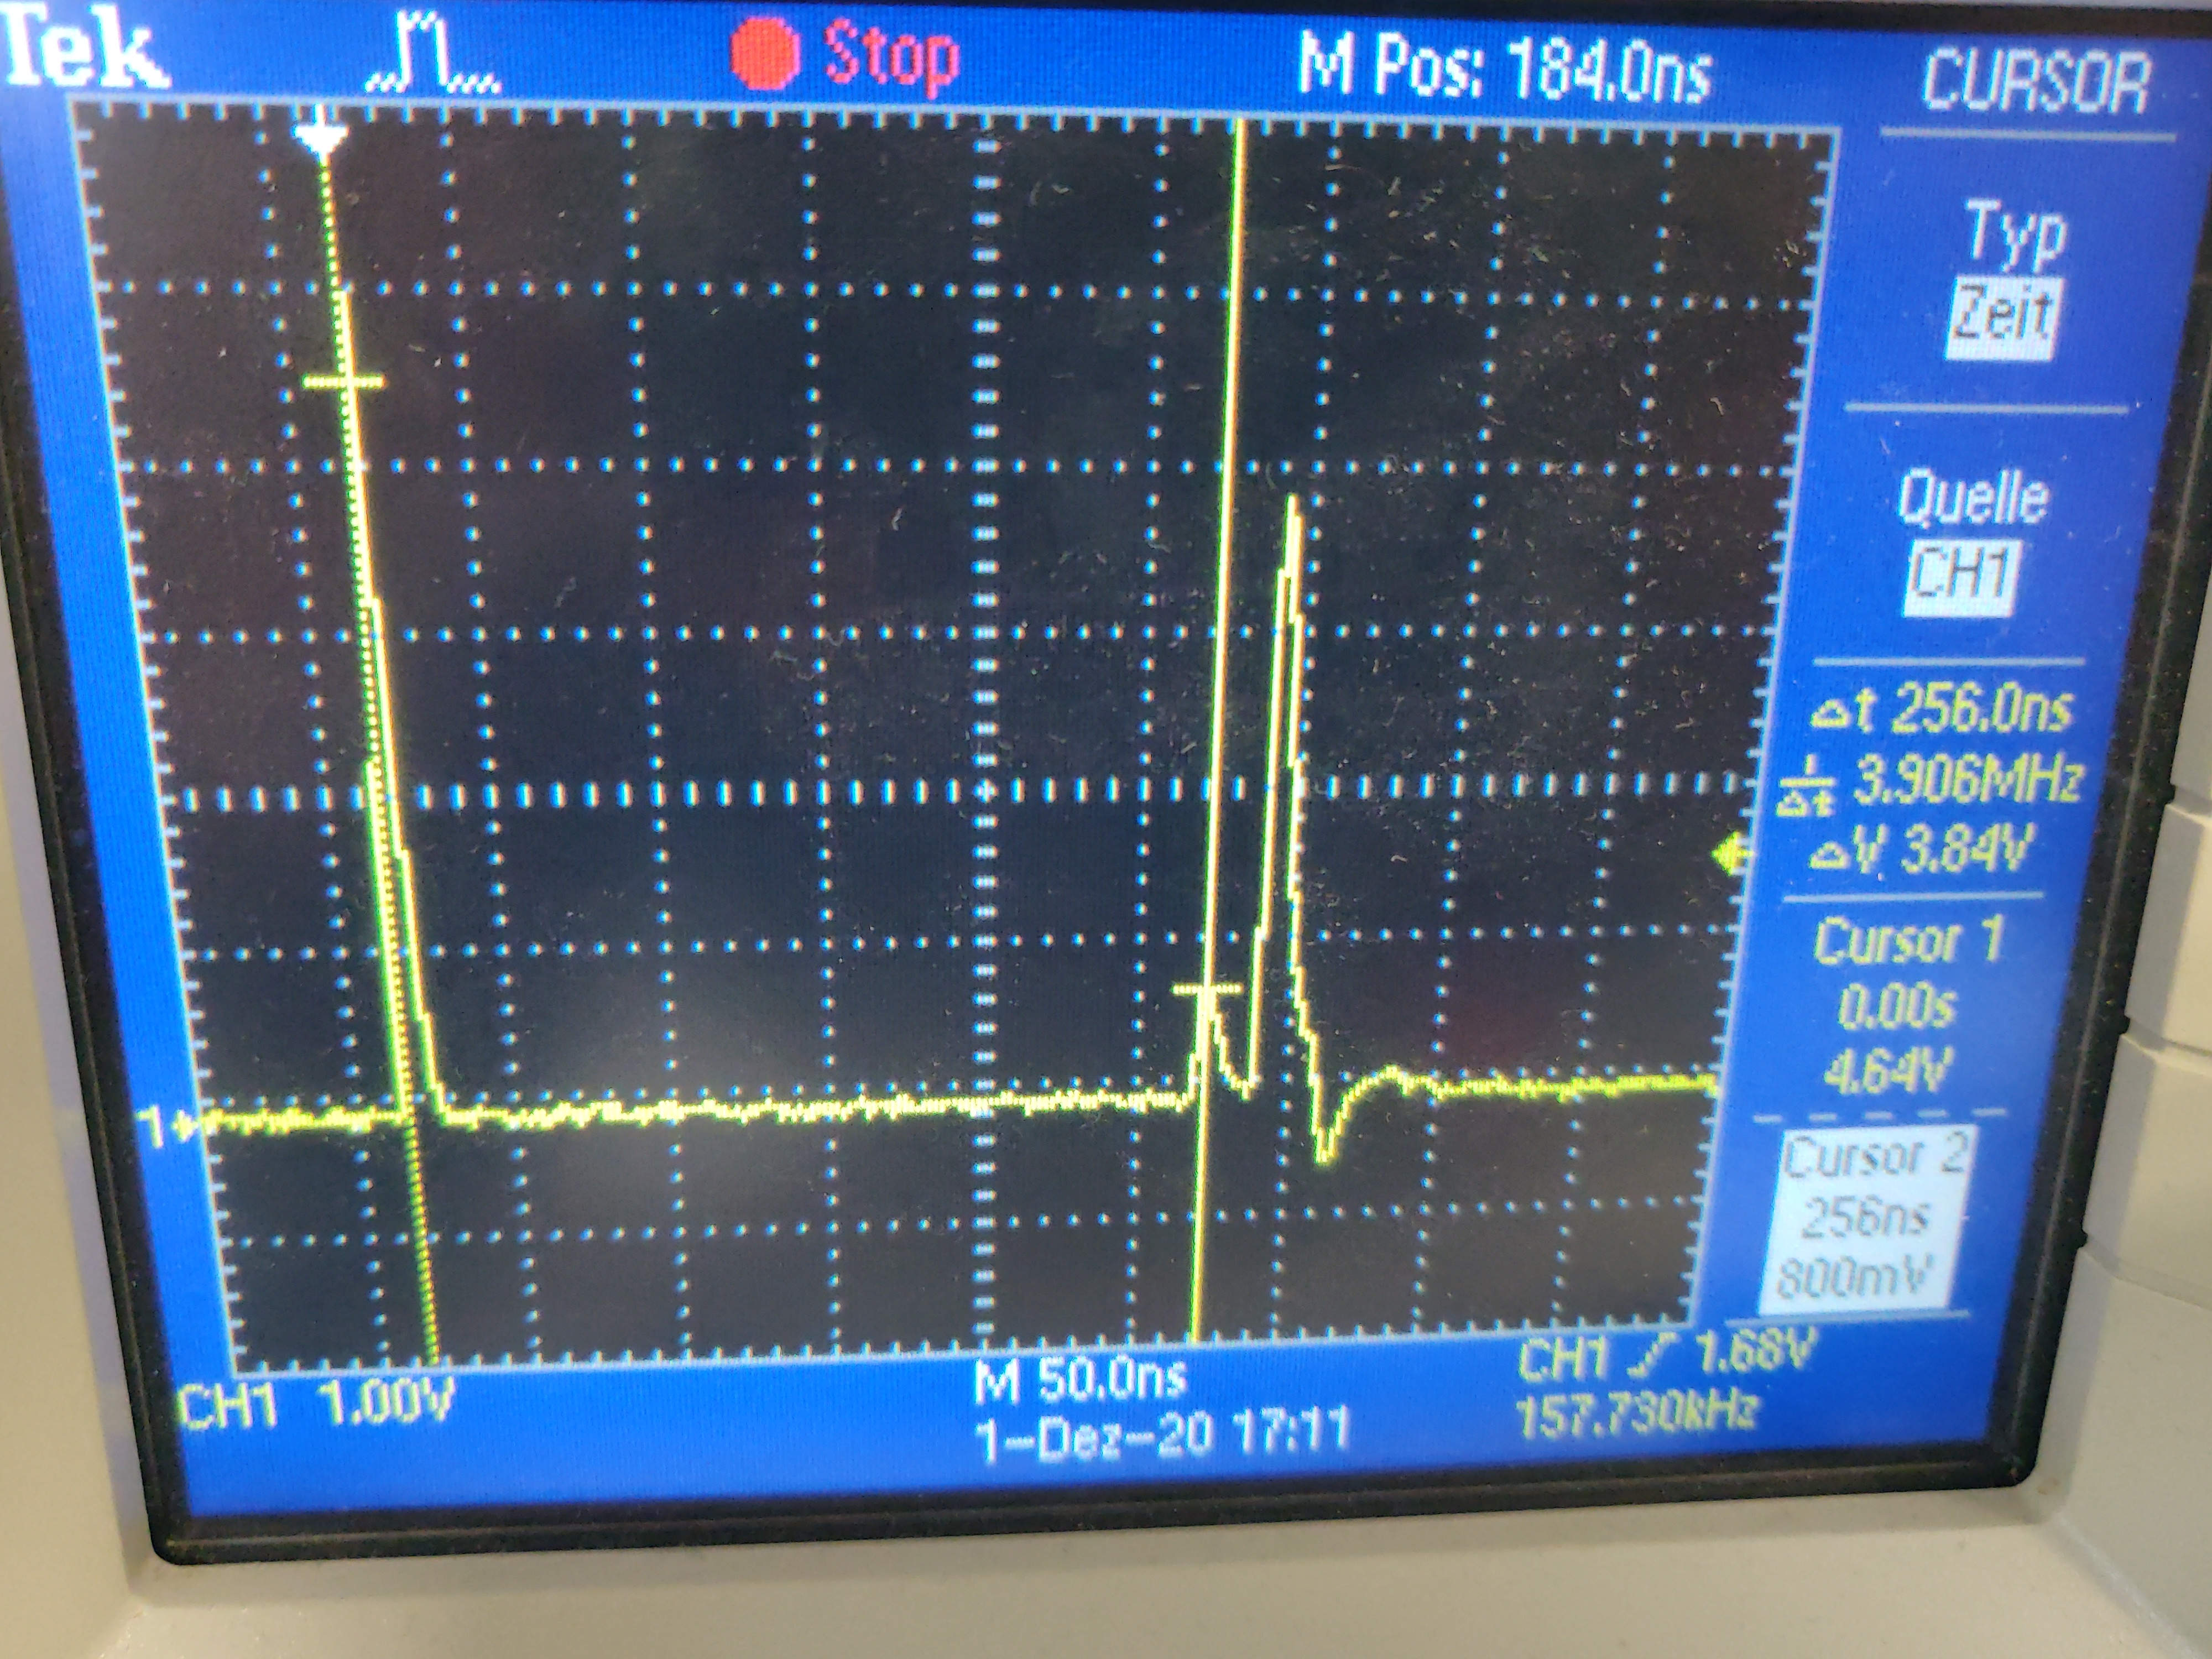
\includegraphics[width=0.45\linewidth]{messdaten/3-3-3_lengthToDefect.jpg}}%
    \hspace{.05\linewidth}
    \subfloat[The length of a transmission line can be deducted by the property of a signal traversing the transmission line at a finite and unaltered speed.\label{subfig:osci:3-3-3_overallLength}]{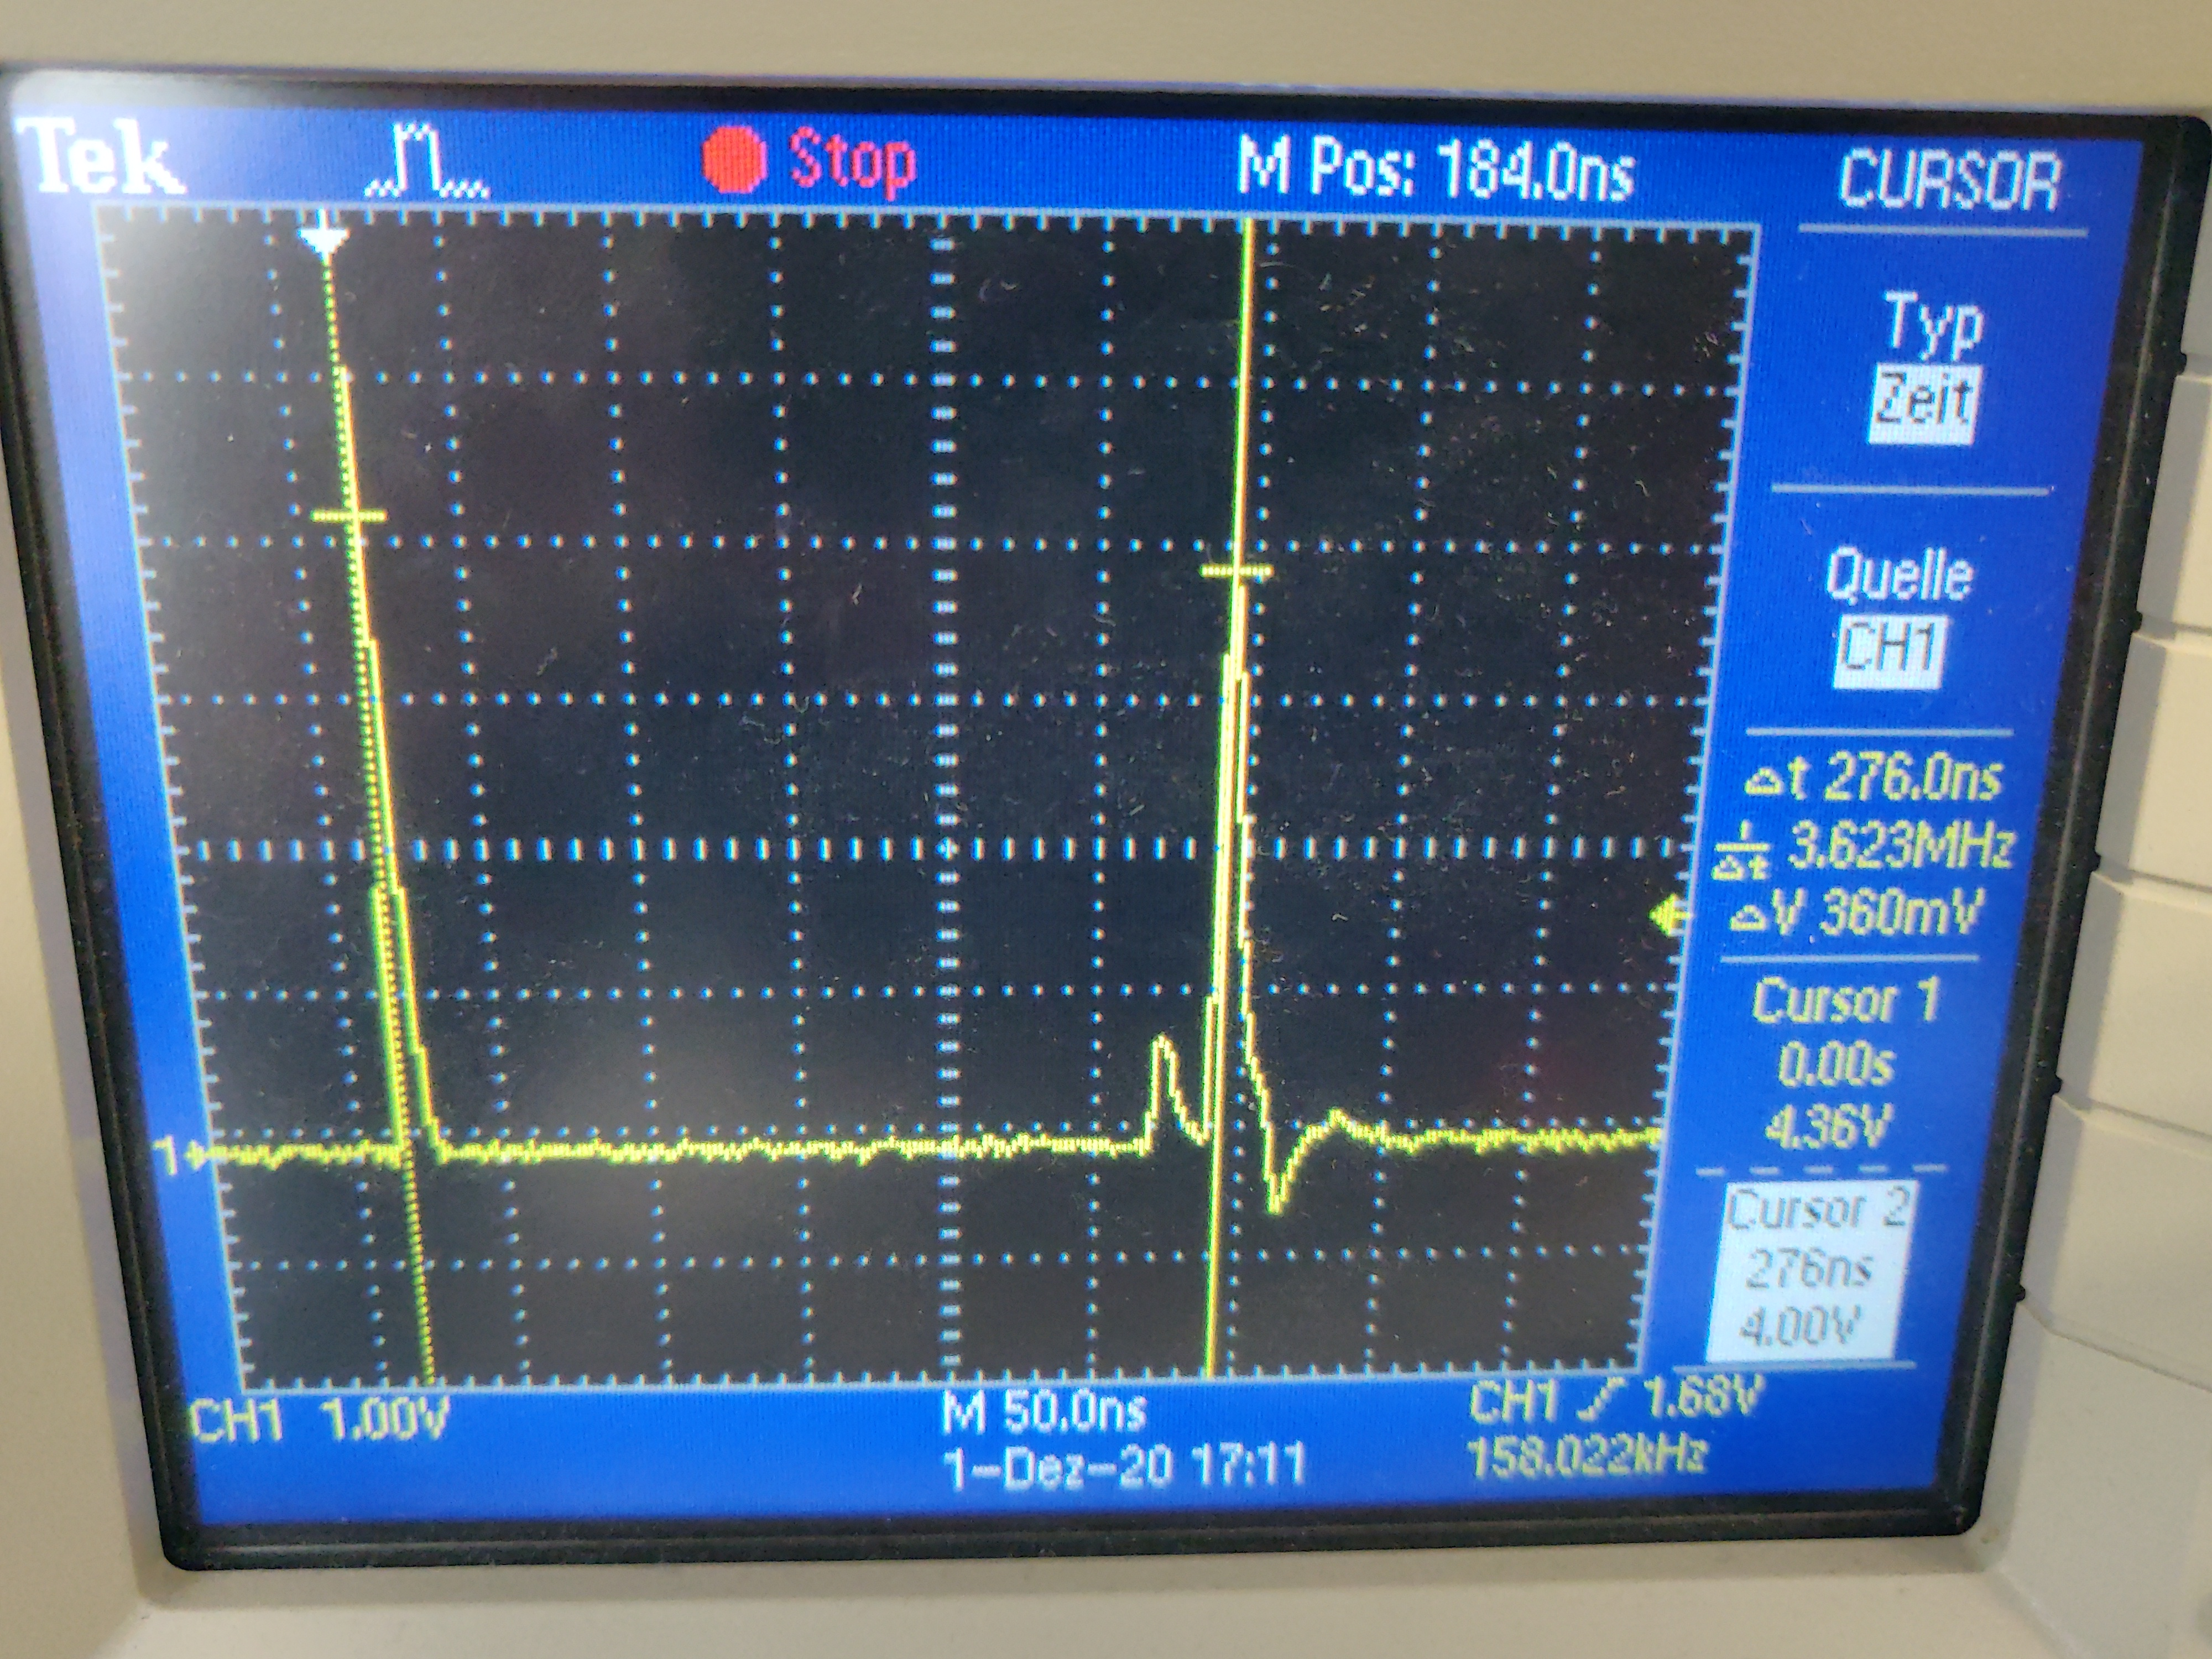
\includegraphics[width=0.45\linewidth]{messdaten/3-3-3_overallLength.jpg}}%
    % \hspace{.05\linewidth}
\end{figure}
\begin{figure}[h]\ContinuedFloat
    \subfloat[Avalanche pulse signal at $ U_{min} $.\label{subfig:osci:avalanche_pulse_signal}]{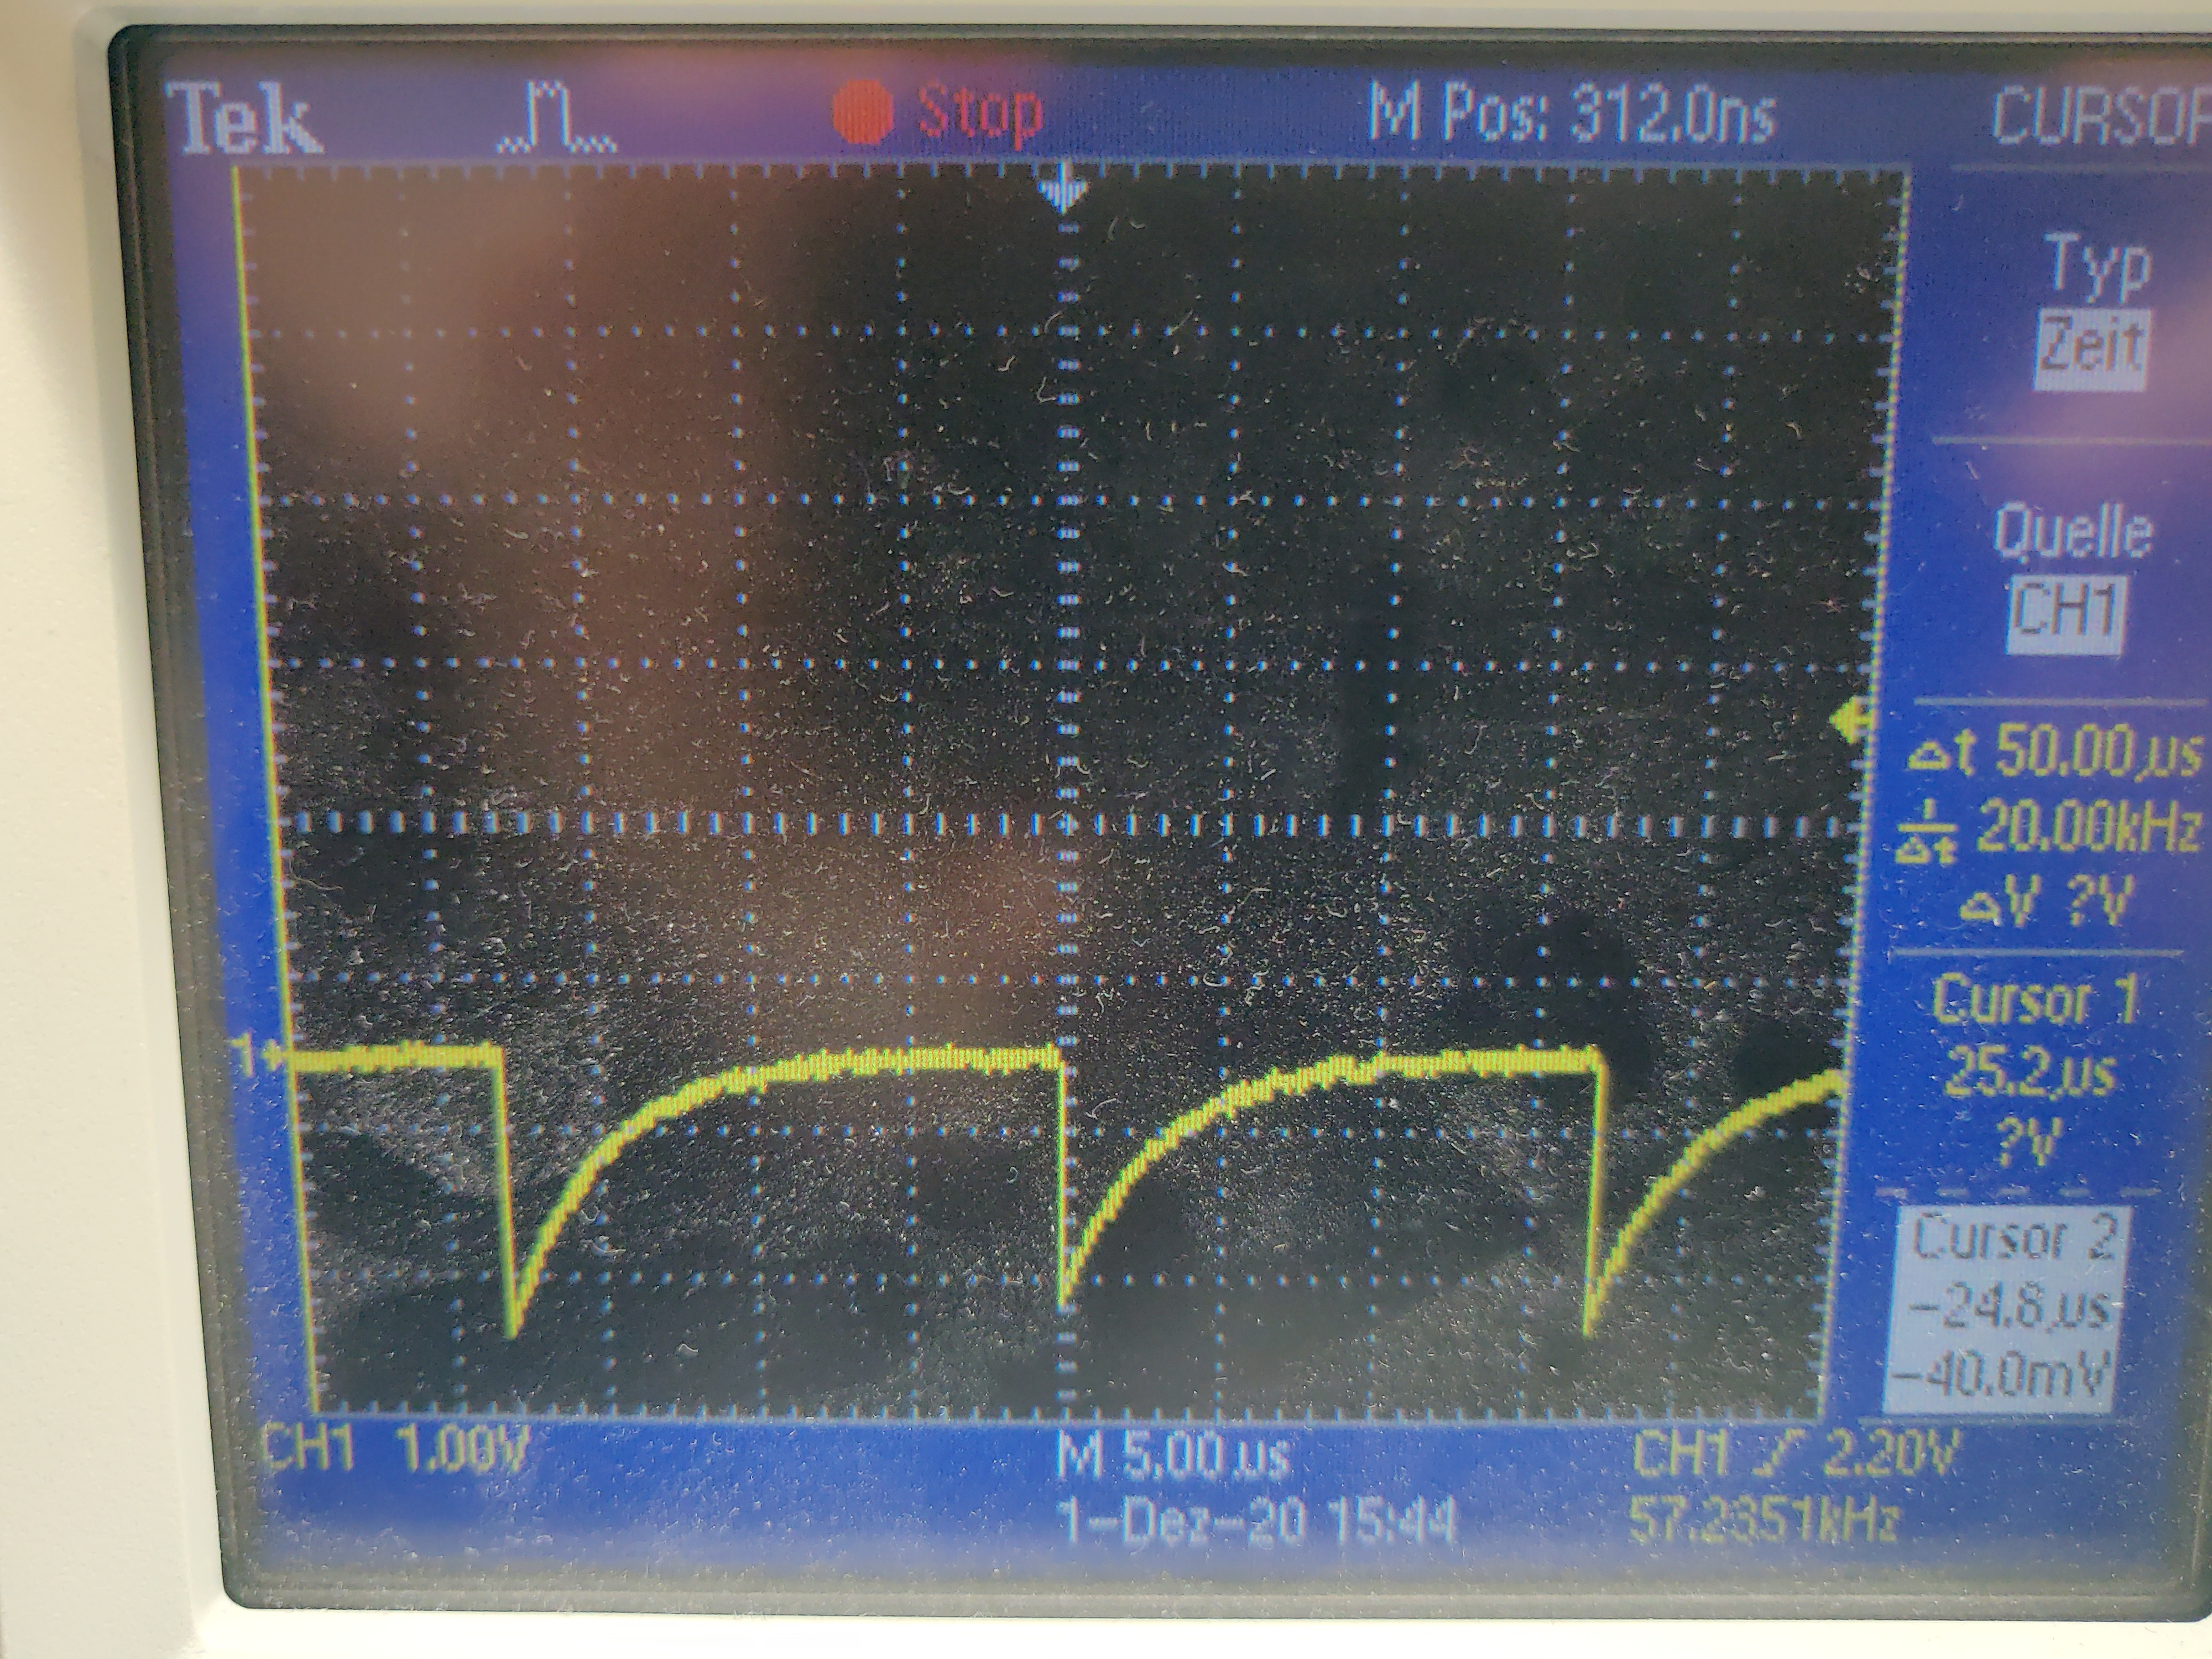
\includegraphics[width=0.45\linewidth]{messdaten/avalanche_pulse_signal.jpg}}%
    \hspace{.05\linewidth}
    \subfloat[Pulse characteristics.\label{subfig:osci:pulsuntersuchung}]{\includegraphics[width=0.45\linewidth]{messdaten/pulsuntersuchung.jpg}}%
    \caption[Oscillograms]{During the course of the experiment captured oscillograms.}%
    \label{fig:oscillograms}
\end{figure}
%
\newpage
%
\begin{table}
    \centering
    \caption[Handwritten notes]{Handwritten notes corresponding each measurement.}%
    \begin{tabular}{cc}
        \adjustbox{valign=t}{
            \subfloat[Duty cycles and measured output voltages at the boost converter.\label{subtab:3-1_duty_vs_voltage}]{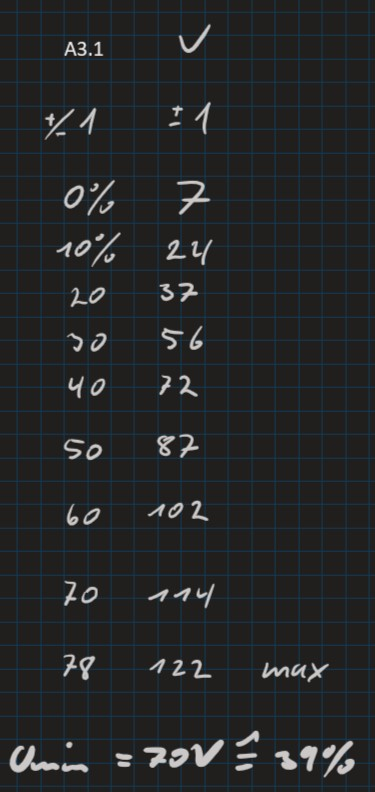
\includegraphics[width=.4\linewidth]{messdaten/handwritten/3-1.jpg}}
            \hspace{.1\linewidth}
        }
        &
        \adjustbox{valign=t}{
            \subfloat[Repetition frequency \( f_{Rep} \) vs. various output voltages.\label{subtab:3-2_duty_vs_repetitionfreq}]{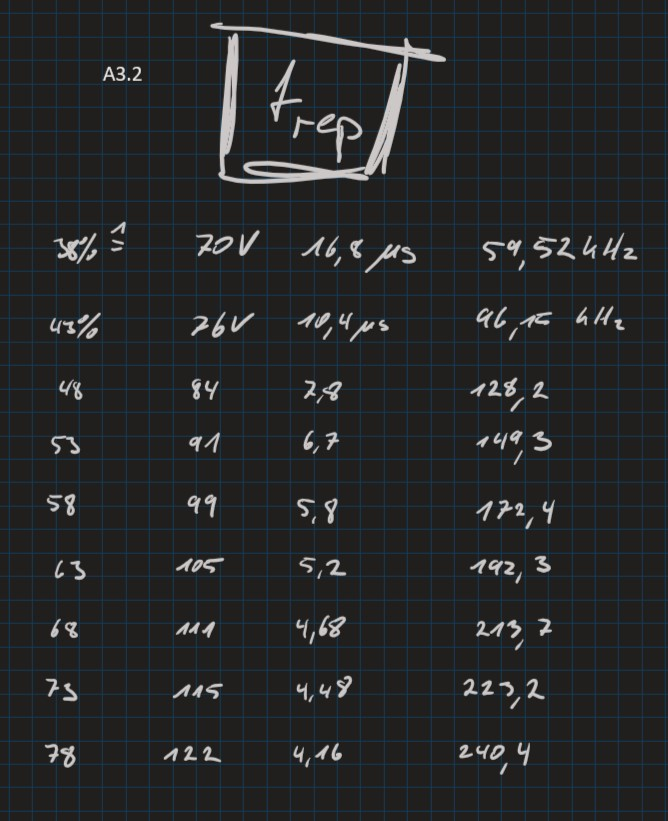
\includegraphics[width=.4\linewidth]{messdaten/handwritten/3-2.jpg}}
            \hspace{.1\linewidth}
        }
    \end{tabular}
\end{table}
\begin{table}
    \ContinuedFloat
    \centering
    % \caption[Handwritten notes]{Handwritten notes corresponding each measurement.}%
    \begin{tabular}{cc}
        \adjustbox{valign=t}{
            \subfloat[Propagation times at three different cable lengths.\label{subtab:3-3-1_propagationTimes_3_cables}]{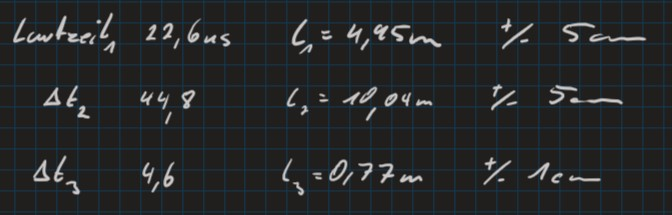
\includegraphics[width=0.4\textwidth]{messdaten/handwritten/3.3.1_propagationTimes.jpg}}%
            \hspace{.1\linewidth}
        }
        &
        \adjustbox{valign=t}{
            \subfloat[Measured impedance of the cables.\label{subtab:3.3.2_cableImpedances}]{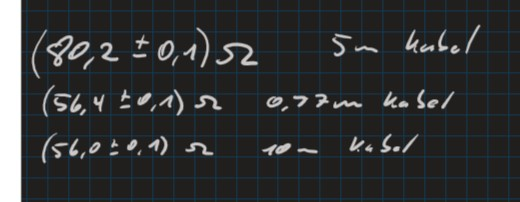
\includegraphics[width=0.4\textwidth]{messdaten/handwritten/3.3.2_cableImpedances.jpg}}%
            \hspace{.1\linewidth}
        }
    \end{tabular}
\end{table}
\begin{table}
    \ContinuedFloat
    \centering
    % \caption[Handwritten notes]{Handwritten notes corresponding each measurement.}%
    \subfloat[Table of the measured cable characteristics.\label{subtab:3.3.2_cableCharacteristicsTable}]{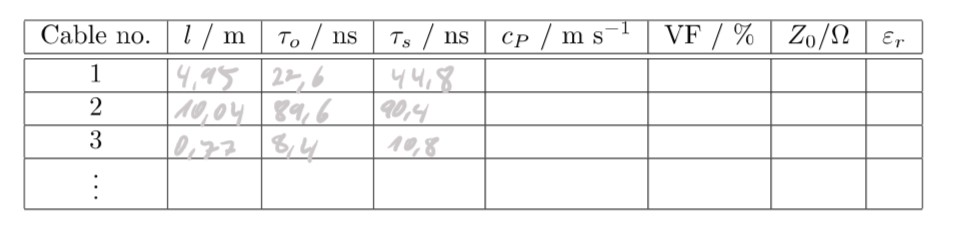
\includegraphics[width=0.6\linewidth]{messdaten/handwritten/3.3.2_cableCharacteristicsTable.jpg}}
\end{table}
%\bibliography{Z:/Dokumente/HSRM/LaTex_Quellen/HSRM_Quellen/quellen}
\printbibliography
%\bibliographystyle{plaindin}
%==========================================
\end{document}